\chapter{Presenting Experimental Images Honestly}

Su, a graduate student in cell biology, was preparing a manuscript on a high-content phenotypic screen of small-molecule compounds. For the supplementary methods section, she needed a figure illustrating the baseline staining quality of nuclei and mitochondria in human osteosarcoma cells (U2OS) from a dimethyl sulfoxide (DMSO) vehicle-control well. She copied several micrographs off the imaging workstation, dragged them into a slide presentation program, and pulled the brightness and contrast sliders until the dim mitochondrial panel ``looked clear.'' She then took a screen capture of the slide and uploaded the screenshot to a generative image tool with the prompt: ``Denoise, sharpen, and upscale to high resolution.''

At lab meeting, her advisor did not comment on how crisp the panels looked. Instead, she asked three questions. First, where are the unmodified 16-bit raw files stored? Second, which exact intervals of raw greyscale values were mapped to black and white in the nuclear and mitochondrial channels, and were the control fields displayed with the exact same intensity window? Third, from which objective magnification and camera pixel size was that ``$20\ \mu\text{m}$'' scale bar in the lower right corner calculated? Su could not answer any of the three. Taking a screenshot had permanently crushed the 16-bit measurements into 8-bit RGB values; the slide sliders left no numerical record of the transfer function; and the scale bar had been drawn by eye to resemble a figure from another paper.

Experimental images differ fundamentally from the workflow diagrams of Chapter~6 and the mechanism schematics of Chapter~7: \textbf{an experimental image is a measurement, not an illustration.} Whether the file comes from a fluorescence microscope, a scanning electron microscope (SEM), a Western blot imager, or a pathology scanner, the numerical value stored at each pixel records the photon or electron count registered by a detector at a defined spatial coordinate. When preparing evidentiary images for publication, AI tools serve only three supporting roles: helping organize a presentation plan, drafting deterministic scripts that read raw arrays and assemble panels without altering source files, and running technical checks on exported figures for file format, resolution, and colour-vision accessibility. \textbf{Generative AI must never touch the pixel values of an evidentiary image.} Using two classes of openly licensed raw micrographs---multichannel fluorescence images of cultured cells and SEM images of plant leaf epidermis---this chapter walks through raw-file stewardship, intensity display mapping, pseudo-colour selection, cropping, scale-bar calibration, journal image-integrity policies, and verifiable delivery logs.

\section{Raw Images Are Evidence: Data, Display, and Export}

In every digital imaging system, \textbf{raw data, display settings, and exported images} are three distinct entities. Confusing what appears on a monitor with what is stored in the file is the root cause of most accidental image distortion and compliance failures.

When a scientific camera---such as an sCMOS or CCD detector---captures a fluorescence micrograph, photons striking each photosite are converted into photoelectrons and quantized by an analogue-to-digital converter (ADC) into integer grey levels. Depending on the hardware, each pixel is digitized at 12 bits ($0\text{--}4095$), 14 bits ($0\text{--}16383$), or 16 bits ($0\text{--}65535$) and saved inside an uncompressed TIFF container or native instrument format (such as OME-TIFF, ND2, CZI, or LIF) paired with acquisition metadata. That two-dimensional integer matrix is the primary measurement.

Standard monitors, web browsers, and PDF viewers, however, display only 8 bits per colour channel ($256$ grey levels, from $0$ to $255$). To render a 16-bit array on an 8-bit screen, viewing software must execute a \textbf{display mapping}: it chooses a lower bound (the black point, $v_{\min}$) and an upper bound (the white point, $v_{\max}$), renders every pixel with $I \le v_{\min}$ as pure black ($0$), renders every pixel with $I \ge v_{\max}$ as pure white ($255$), and scales intermediate values across $[0, 255]$. Under a linear display mapping, the 8-bit displayed grey level $I_{\text{disp}}$ for a raw pixel value $I$ is
\[
I_{\text{disp}} = \operatorname{clip}\!\left(\frac{I - v_{\min}}{v_{\max} - v_{\min}},\, 0,\, 1\right) \times 255.
\]
So long as the source file is not overwritten, changing $v_{\min}$ and $v_{\max}$ only shifts the viewing window; the integer matrix inside the TIFF file remains untouched. Once a researcher clicks ``Save As 8-bit PNG/JPEG'' or takes a screenshot, however, the display mapping is baked irreversibly into the pixel values: measurements outside $[v_{\min}, v_{\max}]$ are permanently clipped, and the 12- or 16-bit dynamic range is collapsed into $256$ discrete steps.

We illustrate this distinction using primary micrographs from the Broad Bioimage Benchmark Collection dataset BBBC022v1 (Gustafsdottir et al., 2013; Ljosa et al., 2012; dedicated to the public domain under CC0~1.0 by Anne Carpenter). Our fluorescence material comes from plate 20585, well A13 (a DMSO vehicle-control well marked \texttt{mock} in the metadata), site~1 (\texttt{s1}) and site~2 (\texttt{s2}), comprising two single-channel files per site: channel \texttt{w1} records Hoechst~33342 nuclear staining, and channel \texttt{w5} records MitoTracker Deep Red mitochondrial staining. Each file is a $696 \times 520$-pixel 16-bit greyscale TIFF acquired with a $20\times$ objective at $0.656\ \mu\text{m/pixel}$, using a camera with an effective 12-bit ADC depth (ceiling $4095$).

In the raw array of the site~1 nuclear channel (\texttt{w1}), all $361,920$ pixels span $121\text{--}1655$, with a mean of $238.4$, $0.1\text{th}$ and $99.9\text{th}$ percentiles of $132$ and $1236$, and zero pixels at the camera ceiling of $4095$. Figure~\ref{fig:ch08-01} renders this single 16-bit array under three linear display windows alongside the corresponding raw-value histograms.

\begin{figure}[htbp]\centering
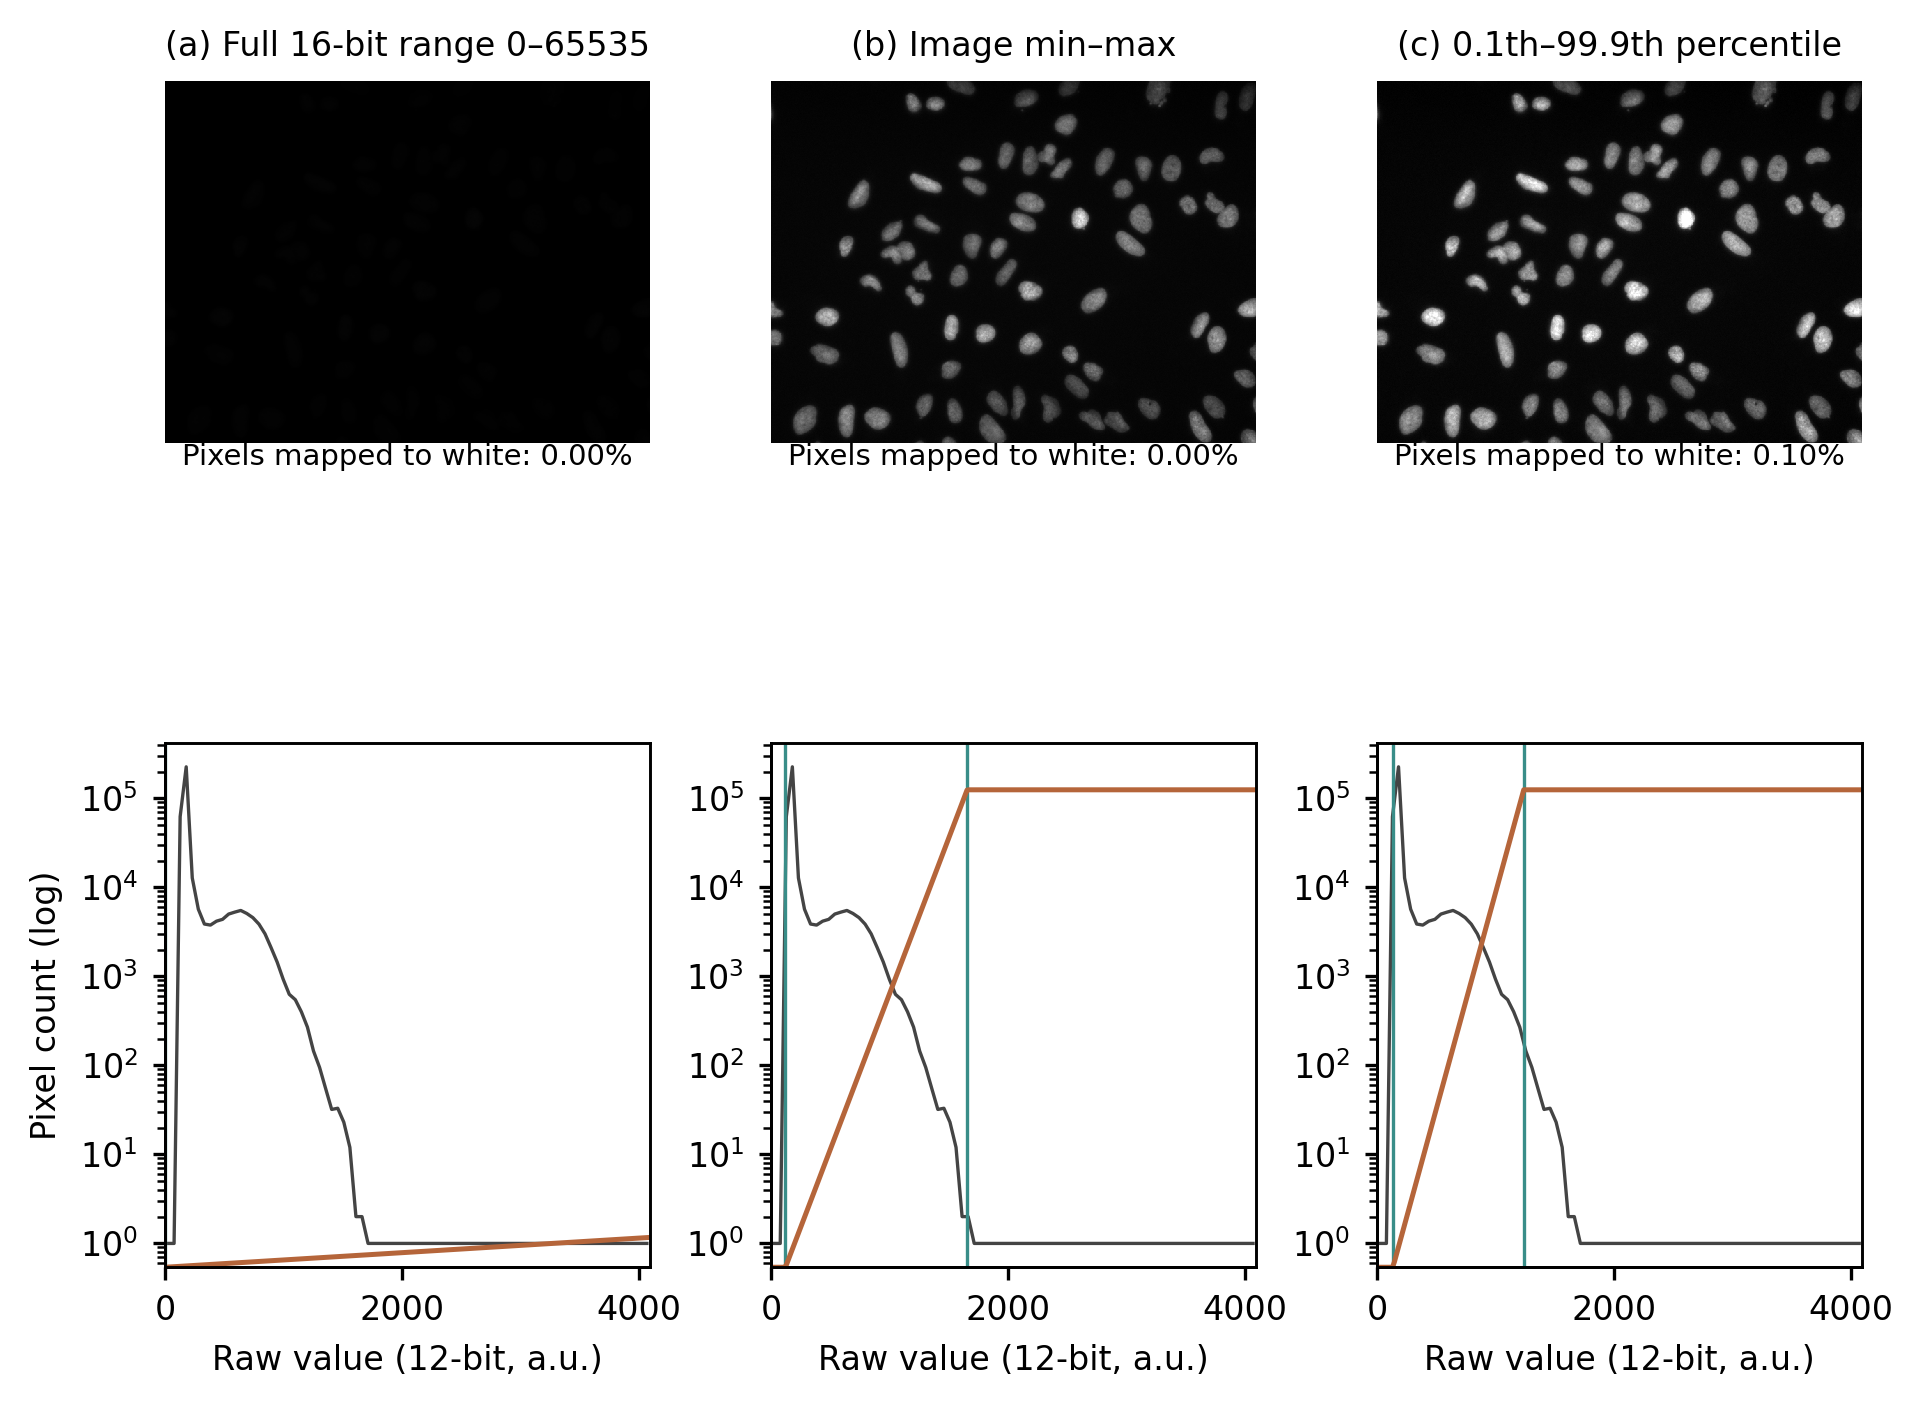
\includegraphics[width=0.88\linewidth]{figures/ch08/ch08-01-raw-display-mapping-en.png}
\caption{One 16-bit fluorescence image (BBBC022, Hoechst channel) shown with three linear display mappings. Raw pixel values are identical in all columns; only the mapping changes: (a) full 16-bit range; (b) image minimum to maximum; (c) $0.1\text{th}$ to $99.9\text{th}$ percentile, with the fraction of pixels mapped to white stated. Bottom: histograms of raw values with the mapping overlaid. Image: BBBC022v1, CC0.}\label{fig:ch08-01}
\end{figure}

Comparing the three columns of Figure~\ref{fig:ch08-01} shows how display mapping governs visual appearance:
\begin{itemize}
\item \textbf{Column (a) (linear mapping across the full 16-bit container range, $0\text{--}65535$):} Generic operating-system viewers map $0$ to black and $65535$ to white when opening a 16-bit TIFF. Because a 12-bit camera never exceeds $4095$ and this field peaks at $1655$, even the brightest pixel maps to $1655 / 65535 \times 255 \approx 6.4$. The top-left panel therefore appears pitch black ($0.00\%$ of pixels mapped to white), and the brown transfer line in the bottom-left plot hugs the horizontal axis. Beginners often mistake this dark window for a failed exposure and overwrite the original file in a photo editor.
\item \textbf{Column (b) (linear mapping from image minimum to maximum, $121\text{--}1655$):} Setting $v_{\min} = 121$ and $v_{\max} = 1655$ (between the two vertical teal lines in the middle histogram) raises the slope of the transfer line, revealing all roughly $60$ nuclei with $0.00\%$ of pixels mapped to white. However, a single condensed, intensely bright nucleus above and to the right of centre pushes the global maximum to $1655$, leaving the remaining interphase nuclei relatively dim.
\item \textbf{Column (c) (linear mapping from the $0.1\text{th}$ to the $99.9\text{th}$ percentile, $132\text{--}1236$):} Setting $v_{\min} = 132$ and $v_{\max} = 1236$ clips only the brightest $0.10\%$ of pixels (concentrated inside that single condensed nucleus) to pure white, spreading the 8-bit greyscale across the interphase population so chromatin texture is clearly resolved.
\end{itemize}

Authors must distinguish two very different kinds of ``pixel ceiling.'' The first is \textbf{display-stage clipping}, as in Figure~\ref{fig:ch08-01}c, where raw values above $1236$ map to $255$ on screen while $1655$ remains intact inside the 16-bit TIFF. The second is \textbf{acquisition-stage sensor saturation} inside the camera ADC. In the site~1 mitochondrial channel (\texttt{w5}), raw pixel values span $185\text{--}4095$ (mean $373.2$, $p_{0.1}/p_{99.9} = 218/1140$), and \textbf{$12$ pixels equal the 12-bit ADC ceiling of $4095$}. Those $12$ pixels overflowed during exposure; no post-processing algorithm can recover their true photon counts. For qualitative methods panels with a few isolated saturated pixels, the honest course is to leave the pixels unaltered and report the count in the catalogue and legend; if saturation affects regions used for intensity quantification, the sample must be re-imaged at shorter exposure.

The first rule of experimental image stewardship follows: \textbf{copy before processing, and lock raw files as read-only.} Store original files in a write-protected directory, compute SHA-256 checksums, and compile a \textbf{raw-image catalogue} recording filename, hash, bit depth, dimensions, physical pixel size, and acquisition metadata. All display mapping and cropping should then run via a deterministic script that reads the read-only masters and writes lossless 8-bit PNG or TIFF display derivatives---never using lossy JPEGs or screenshots as source files. General-purpose AI assistants can write Python scripts to scan directories, compute SHA-256 digests, and count saturated pixels; the author must verify the camera's effective bit depth ($4095$ versus $65535$) and confirm the source of the physical pixel size.

\section{Contrast Adjustments: Linear, Non-Linear, and Disclosed}

Editorial policies at major journals---including the \emph{Journal of Cell Biology} (Rossner and Yamada, 2004) and Nature Portfolio---define four boundaries for contrast adjustments.

\textbf{First, whole-image linear adjustments are permitted, provided they do not obscure or eliminate valid data.} Within $[v_{\min}, v_{\max}]$, subtracting the black point preserves the exact intensity ratio between any two nonsaturated features. Pushing $v_{\min}$ above background to make the background look ``clean,'' or pulling $v_{\max}$ down to make dim features blaze, clips real signal into $0$ or $255$ and erases structural detail.

\textbf{Second, non-linear transfer functions---such as gamma ($\gamma$) correction, logarithmic transforms, or spline curves---alter relative intensity ratios across the dynamic range and must be disclosed in the figure legend.} Under a gamma mapping,
\[
I_{\text{disp}} = \left[\operatorname{clip}\!\left(\frac{I - v_{\min}}{v_{\max} - v_{\min}},\, 0,\, 1\right)\right]^{\gamma} \times 255.
\]
When $\gamma < 1$ (e.g., $\gamma = 0.5$), the transfer curve bows upward, boosting weak signals while compressing bright signals so structures that differ several-fold in raw photon counts appear similar in brightness.

Figure~\ref{fig:ch08-02} quantifies this effect on the site~1 mitochondrial channel (\texttt{w5}) across a linear mapping, a $\gamma = 0.5$ mapping with the same black and white points, and an over-clipped linear counter-example. We fix two $15 \times 15$-pixel regions of interest (ROIs): a bright perinuclear mitochondrial cluster at $(340, 210)\text{--}(355, 225)$ (cyan tick) and a dim peripheral cytoplasmic region at $(120, 380)\text{--}(135, 395)$ (yellow tick). After subtracting the black point ($218$), the ratio of mean raw intensities between the bright and dim ROIs is $3.57$.

\begin{figure}[htbp]\centering
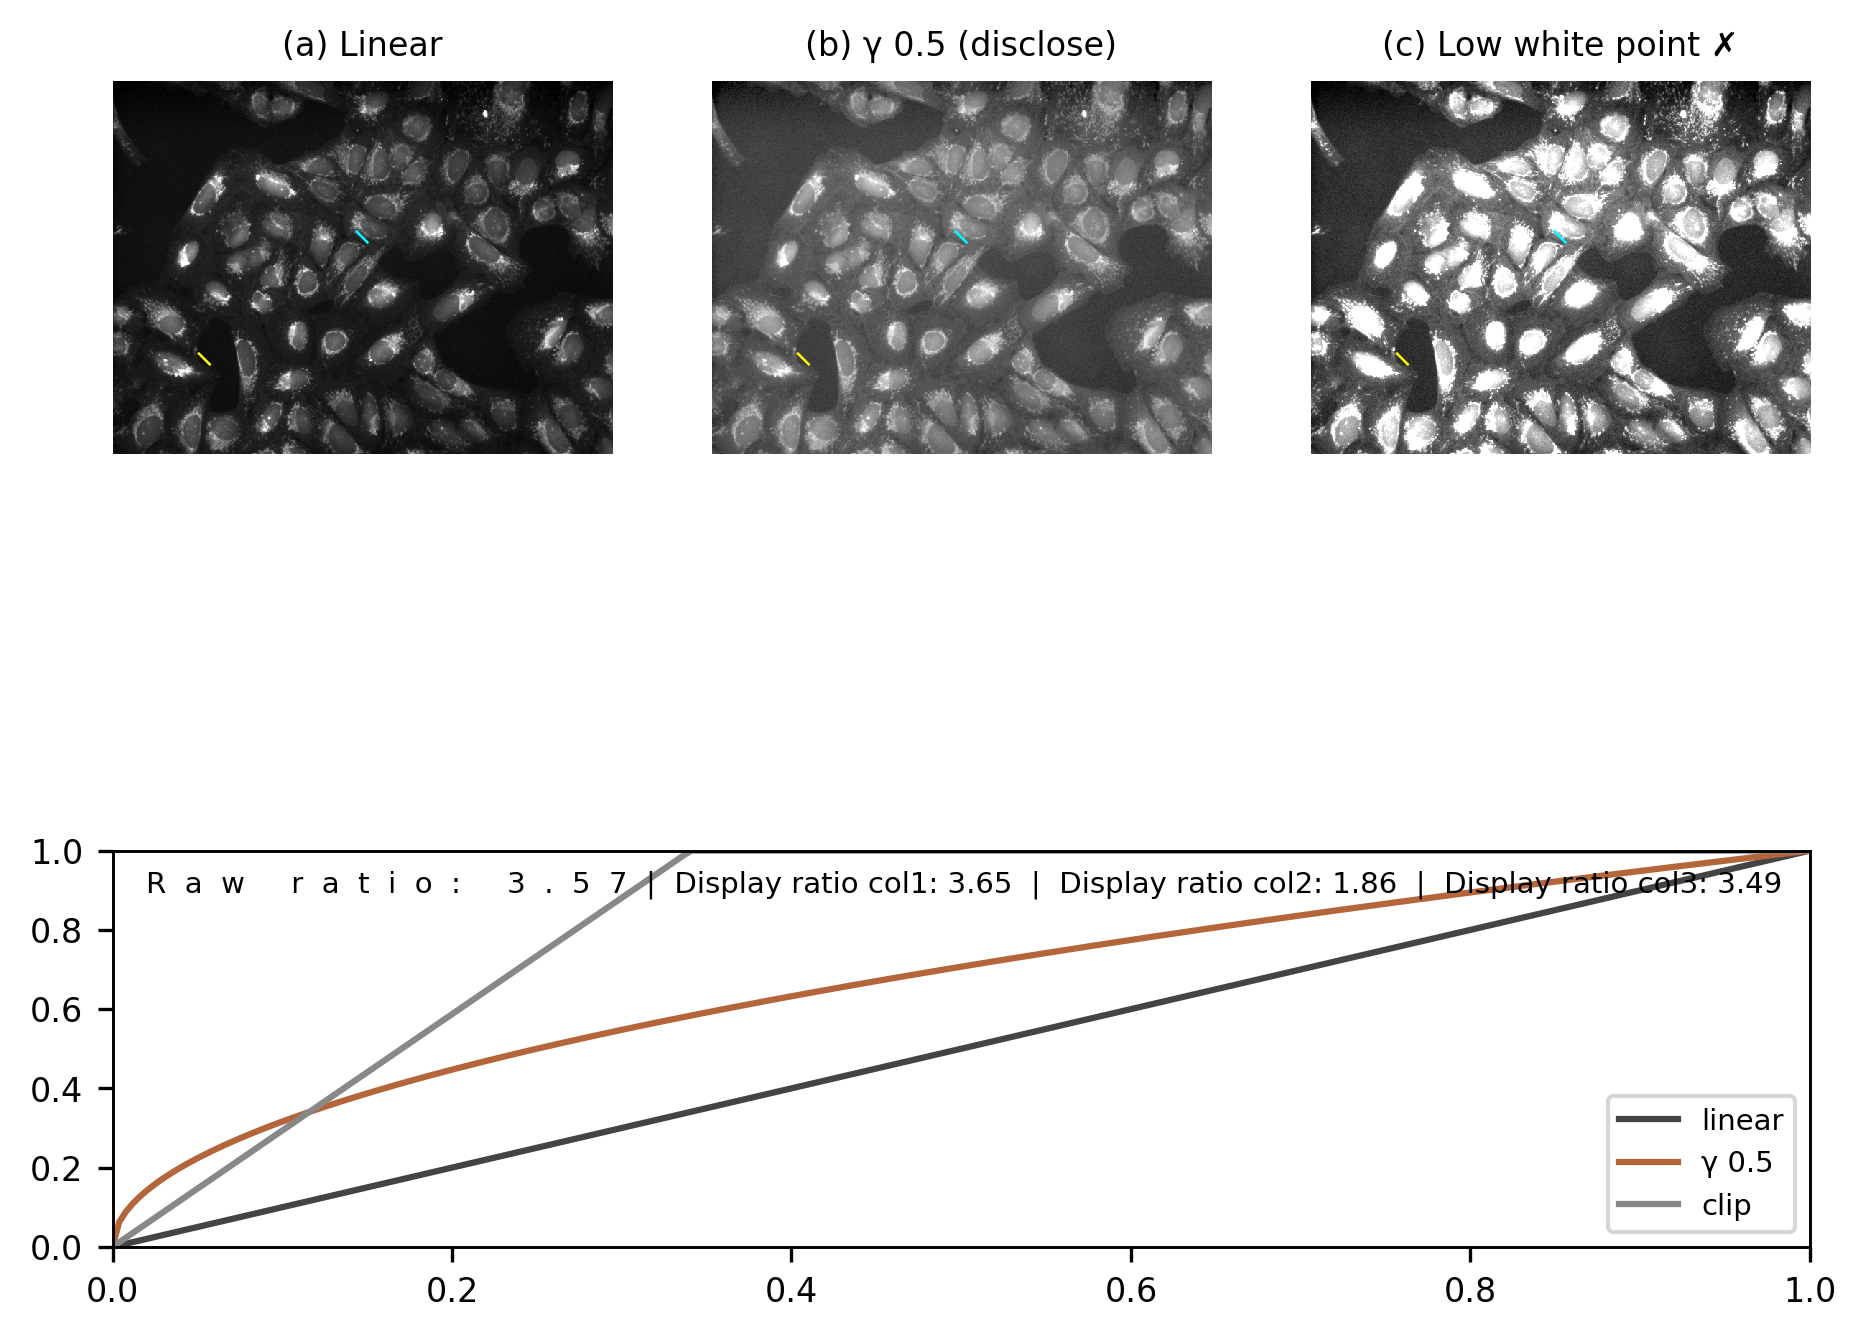
\includegraphics[width=0.88\linewidth]{figures/ch08/ch08-02-linear-vs-gamma-en.png}
\caption{Linear versus non-linear display. (a) Linear mapping ($218\text{--}1140$). (b) The same image with $\gamma = 0.5$: dim signal is brightened and the relative intensity of bright and dim regions changes, so the adjustment must be disclosed. (c) Counter-example: a white point set too low clips most mitochondrial signal to white and destroys information. Curves show the three mappings and list the raw intensity ratio and display grey-level ratios for two fixed regions (cyan and yellow ticks). Image: BBBC022v1, CC0.}\label{fig:ch08-02}
\end{figure}

Inspecting the three columns and transfer curves in Figure~\ref{fig:ch08-02} shows why disclosure is mandatory:
\begin{enumerate}
\item \textbf{Panel (a) (linear mapping, $218\text{--}1140$):} Perinuclear clusters and distal cytoplasmic tubules are resolved in true proportion; the 8-bit displayed grey-level ratio between the cyan and yellow ROIs is $3.65$ (\texttt{Display ratio col1: 3.65}), matching the raw ratio of $3.57$ within integer rounding.
\item \textbf{Panel (b) ($\gamma = 0.5$ over $218\text{--}1140$):} The brown curve arches upward, brightening peripheral tubules, but the displayed ROI ratio drops from $3.57$ to $1.86$ (\texttt{Display ratio col2: 1.86})---nearly halving the apparent contrast. Without disclosing $\gamma = 0.5$ in the legend, readers misjudge the spatial distribution of signal.
\item \textbf{Panel (c) (counter-example: white point lowered to the $90\text{th}$ percentile, $532$):} The grey line hits the ceiling about one-third of the way across the horizontal axis, clipping \textbf{$9.94\%$ of all pixels to pure white ($255$)}. Although the ROI mean ratio numerically reads $3.49$ (\texttt{Display ratio col3: 3.49}, because the steeper slope inflates the dim ROI while clamping the bright ROI at $255$), perinuclear mitochondria collapse into solid white blobs with all internal morphology lost.
\end{enumerate}

\textbf{Third, thresholding backgrounds to zero, local dodging or burning, and clone-stamp or healing-brush retouching are strictly forbidden.} Selectively brightening cells or painting over fluorescent debris falsifies empirical data (Rossner and Yamada, 2004; Cromey, 2010).

\textbf{Fourth, all panels compared within a figure must share identical display settings.} Applying per-panel ``auto-contrast'' cancels out real treatment differences and manufactures fake differences between identical controls. Figure~\ref{fig:ch08-03} demonstrates this using two adjacent fields (\texttt{s1} and \texttt{s2}, mitochondrial channel) from the \emph{same} DMSO control well (well A13). As shown in the right-hand bar chart, the whole-field mean raw intensities of the two 16-bit arrays are nearly identical: $373.2\ \text{a.u.}$ for \texttt{s1} and $366.3\ \text{a.u.}$ for \texttt{s2}, differing by less than $2\%$ (each bar is a single field mean shown to verify baseline magnitude, not a statistical test).

\begin{figure}[htbp]\centering
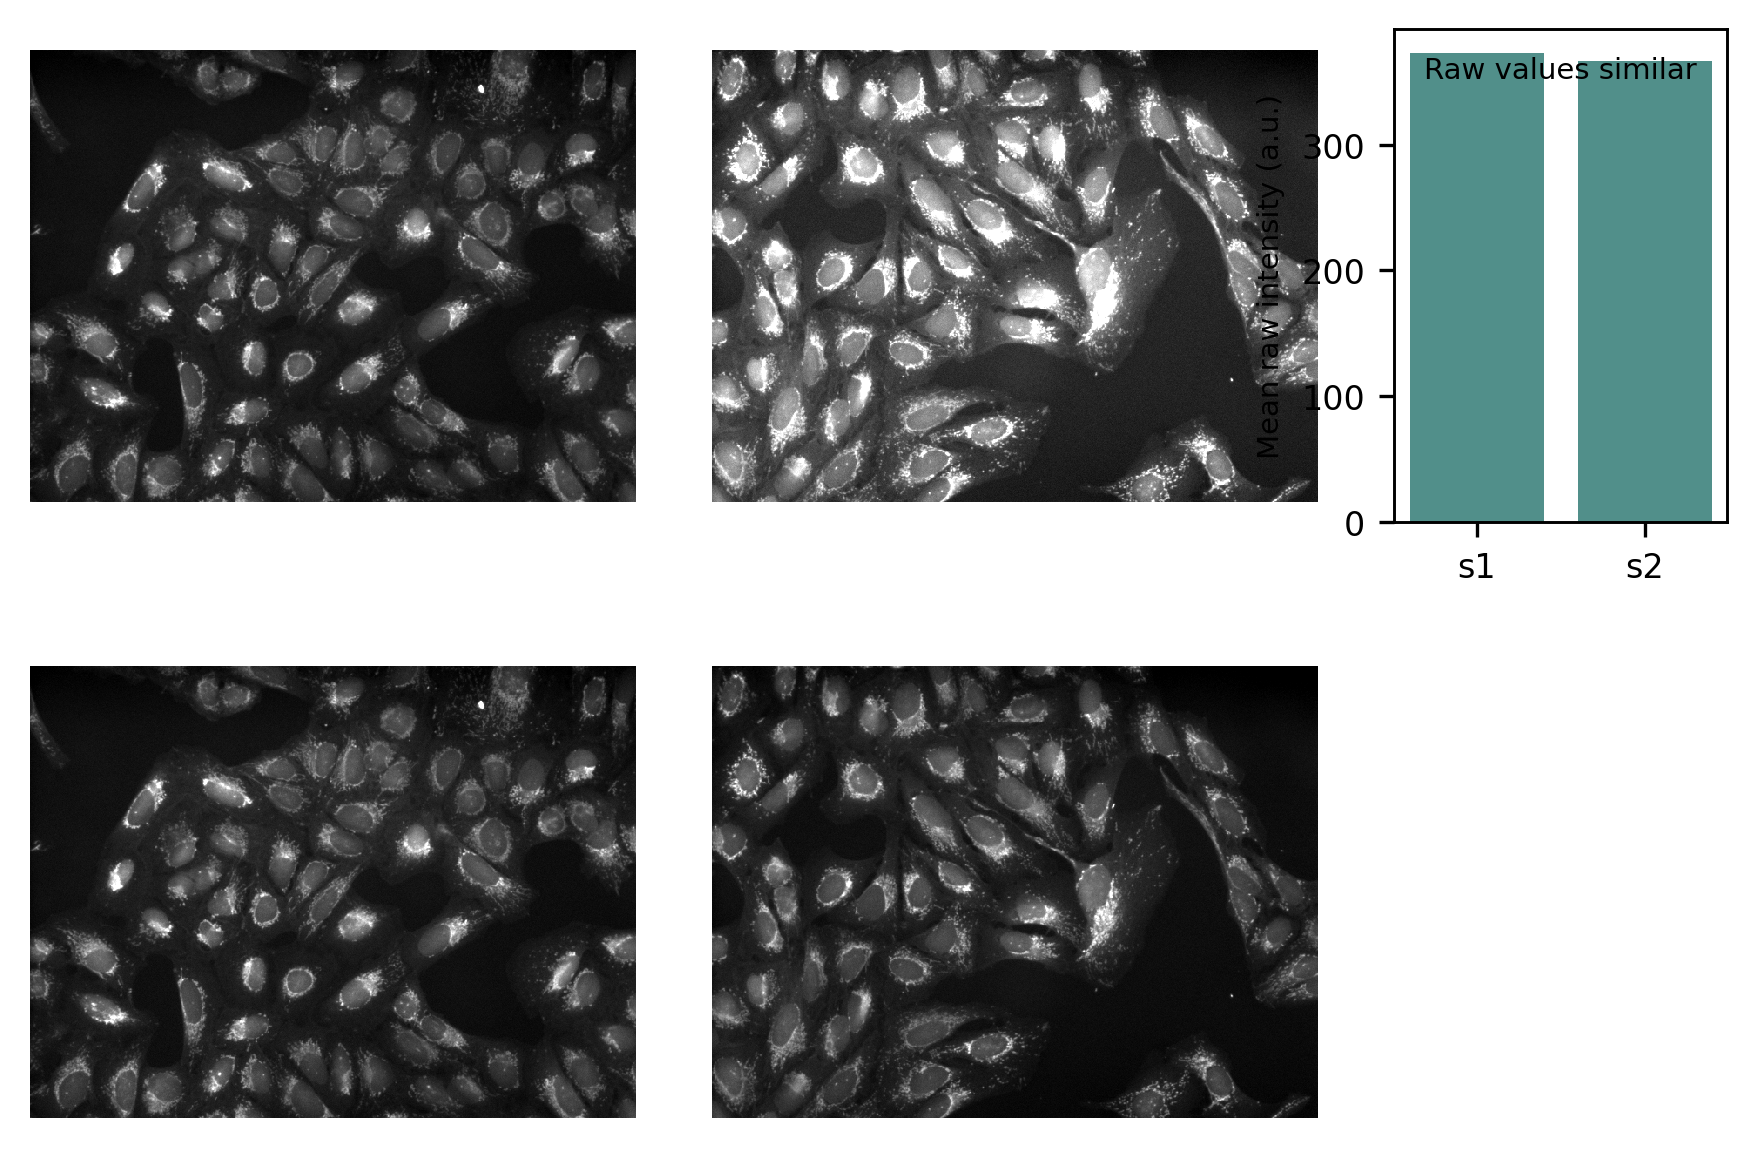
\includegraphics[width=0.88\linewidth]{figures/ch08/ch08-03-consistent-display-en.png}
\caption{Compared panels must share display settings. Both images come from the same control well (BBBC022, well A13, sites~1 and~2) with no treatment difference. Top: display ranges set separately, so the right image appears brighter. Bottom: one shared range ($218\text{--}1140$), and the apparent difference disappears. Right: mean raw intensity of the two fields. The top-right display range was chosen deliberately as a counter-example. Image: BBBC022v1, CC0.}\label{fig:ch08-03}
\end{figure}

In the top row of Figure~\ref{fig:ch08-03}, \texttt{s1} is mapped over $218\text{--}1140$ while \texttt{s2} has its white point lowered to $196\text{--}700$. Lowering the white point by $39\%$ makes the right panel blaze with bright mitochondria, mimicking a strong treatment effect; in the bottom row, applying the shared range $218\text{--}1140$ restores visual parity.

\section{Channels and Pseudo-Colour}

Monochrome fluorescence cameras capture each emission band as a single-channel greyscale array; the colours seen in figures are lookup tables (LUTs) chosen by the author. Selecting channel LUTs follows three rules.

\textbf{First, avoid red/green merges; use magenta/green (or cyan/magenta/yellow) and provide split-channel greyscale panels.} Roughly $8\%$ of male readers have red--green colour-vision deficiency (Wong, 2011; Crameri et al., 2020). In a red/green overlay, pure red ($R$) and pure green ($G$) project onto similar yellow-brown hues under deuteranopia or protanopia, making the two channels and yellow ($R+G$) colocalization regions hard to tell apart. Mapping the first channel to \textbf{magenta} (writing identical 8-bit grey values into both red $R$ and blue $B$) and the second to \textbf{green} ($G$) adds a strong short-wavelength blue component, and overlapping signal sums to high-contrast white ($R+G+B$), remaining separable under both deuteranopia and protanopia. Moreover, human vision resolves fine spatial detail better in single-channel greyscale than in colour (Schmied and Jambor, 2020; Jambor et al., 2021), making ``split-channel greyscale + magenta/green merge'' the safest combination.

Figure~\ref{fig:ch08-04} tests both palettes on a $300 \times 300$-pixel crop from site~1 ($(198, 110)\text{--}(498, 410)$, with display windows fixed at $132\text{--}1236$ for nuclei and $218\text{--}1140$ for mitochondria), simulating colour-vision deficiency in linear sRGB space with the model of Machado et al.\ (2009) at severity $1.0$.

\begin{figure}[htbp]\centering
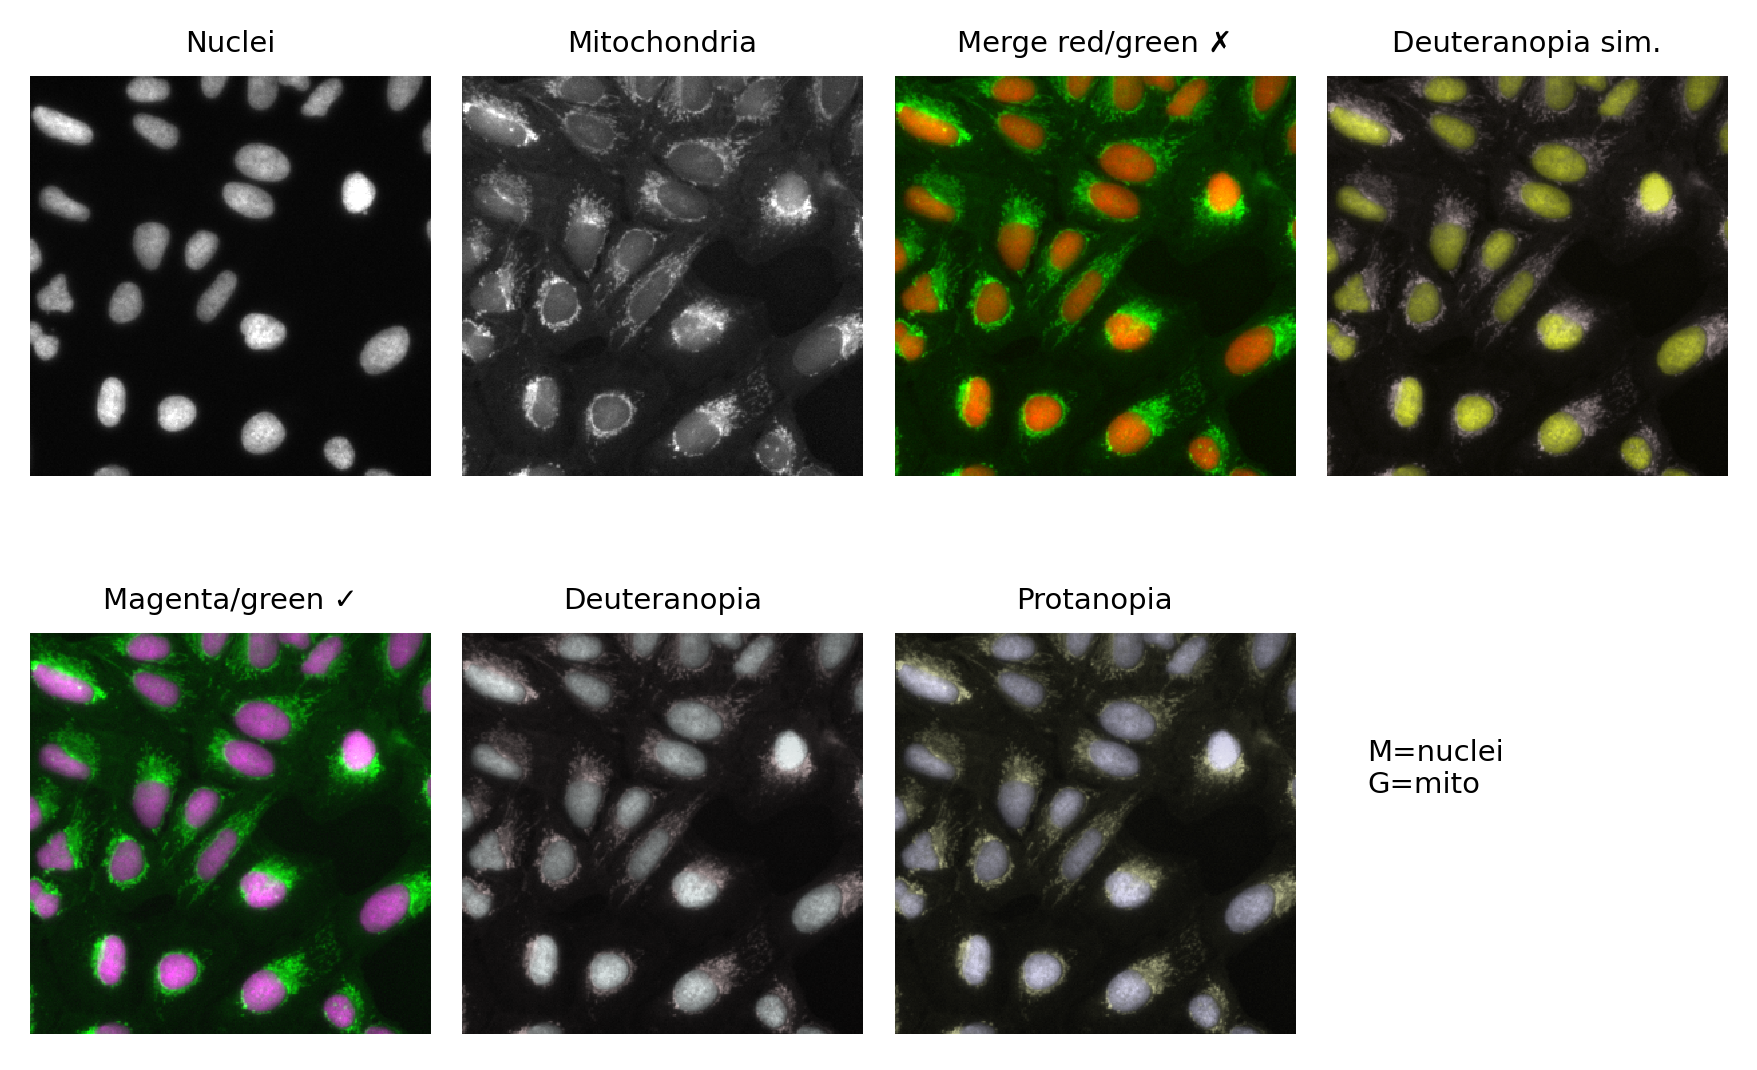
\includegraphics[width=0.88\linewidth]{figures/ch08/ch08-04-pseudocolor-colorblind-en.png}
\caption{Choosing pseudo-colours for multichannel fluorescence. Top: in a red/green merge the two channels become hard to tell apart under simulated deuteranopia. Bottom: a magenta/green merge stays distinguishable under simulated deuteranopia and protanopia. Single-channel greyscale panels need no colour discrimination. Simulation after Machado et al.\ (2009). Image: BBBC022v1, CC0.}\label{fig:ch08-04}
\end{figure}

In the top row of Figure~\ref{fig:ch08-04}, the red/green merge (third column) collapses under simulated deuteranopia (fourth column) into uniform olive-yellow across both nuclei and mitochondria. In the bottom row, the magenta/green merge (first column) preserves clear contrast between slate-violet nuclei and warm olive mitochondria under both simulated deuteranopia (second column) and protanopia (third column). After exporting a figure, authors can also run the \scidraw{} Figure Checker (\sdtool{figure-checker}) to check for colour-vision risks.

\textbf{Second, set and log each channel's linear display range independently before merging.} Nature Portfolio policies require disclosing single-channel adjustments inside a merged image. Mapping each 16-bit channel to 8-bit greyscale via fixed $(v_{\min}, v_{\max})$ bounds in a script before stacking RGB channels---without post-merge colour curves---keeps every parameter exact and reportable.

\textbf{Third, scanning electron micrographs have no native colour; artificial colouration is pseudo-colour and must be declared.} Electron detectors record electron flux as single-channel greyscale. For example, in the public-domain mixed-pollen SEM pair from the Dartmouth Electron Microscope Facility, the archival original (\url{https://commons.wikimedia.org/wiki/File:Misc_pollen.jpg}, $1228 \times 935$ pixels) is greyscale, whereas the colourised version (\url{https://commons.wikimedia.org/wiki/File:Misc_pollen_colorized.jpg}) was hand-tinted afterwards by grain outline. As experimental evidence, SEM images should remain greyscale; if pseudo-colour is applied for illustration, the legend must state that the colours are artificial.

\section{Cropping, Insets, and Scale Bars}

\subsection{Meaning-Preserving Cropping and Zoomed Insets}

Cropping focuses attention on relevant structures, but it must never become ``cherry-picking the brightest or prettiest cell in the field'' (Cromey, 2010; Jambor et al., 2021). Compliant cropping and inset magnification require four practices:
\begin{enumerate}
\item \textbf{Select a representative region and document the criterion:} For a control field, choose a subregion whose nuclear and mitochondrial intensities lie near the field medians, and write that rationale into the processing log.
\item \textbf{Log exact crop coordinates:} Save the pixel bounding box $(x_0, y_0, x_1, y_1)$ in the processing log.
\item \textbf{Mark inset locations on the parent panel and use integer-multiple nearest-neighbour sampling:} Draw a bounding box on the parent image at the exact crop coordinates and state the zoom factor (e.g., $3\times$). Enlarge pixel patches with \textbf{nearest-neighbour interpolation}, expanding each raw pixel into a $k \times k$ block of identical values so the detector's spatial sampling limit remains visible, rather than smoothing edges with bicubic interpolation or ``inventing detail.''
\item \textbf{Never splice separate fields seamlessly:} Images from different fields, time points, or gel lanes must never be abutted to look like one continuous acquisition; legitimate juxtapositions require a clear dividing line and explanation in the legend (Rossner and Yamada, 2004; Bik et al., 2016).
\end{enumerate}

\subsection{Calculating Scale Bars from Calibration Metadata}

The pixel length of a scale bar equals the target physical length divided by the physical pixel size, $L_{\text{px}} = L_{\text{phys}} / s_{\text{px}}$; for an inset enlarged by a factor $k$, the scale-bar pixel length scales by $k$: $L'_{\text{px}} = (L'_{\text{phys}} / s_{\text{px}}) \times k$. Physical pixel size $s_{\text{px}}$ may come only from acquisition metadata, a stage micrometer photographed under identical optics, or an \textbf{instrument data bar} burned into the raw file.

Figure~\ref{fig:ch08-05} demonstrates scale-bar derivation, documented cropping, and nearest-neighbour magnification on a public-domain SEM micrograph of \emph{Nicotiana alata} upper leaf epidermis (\path{Leaf_epidermis.jpg}, $2048 \times 2073$ pixels, 8-bit greyscale), acquired on a Zeiss DSM~962 SEM at $200\times$ by Louisa Howard at the Dartmouth Electron Microscope Facility.

\begin{figure}[htbp]\centering
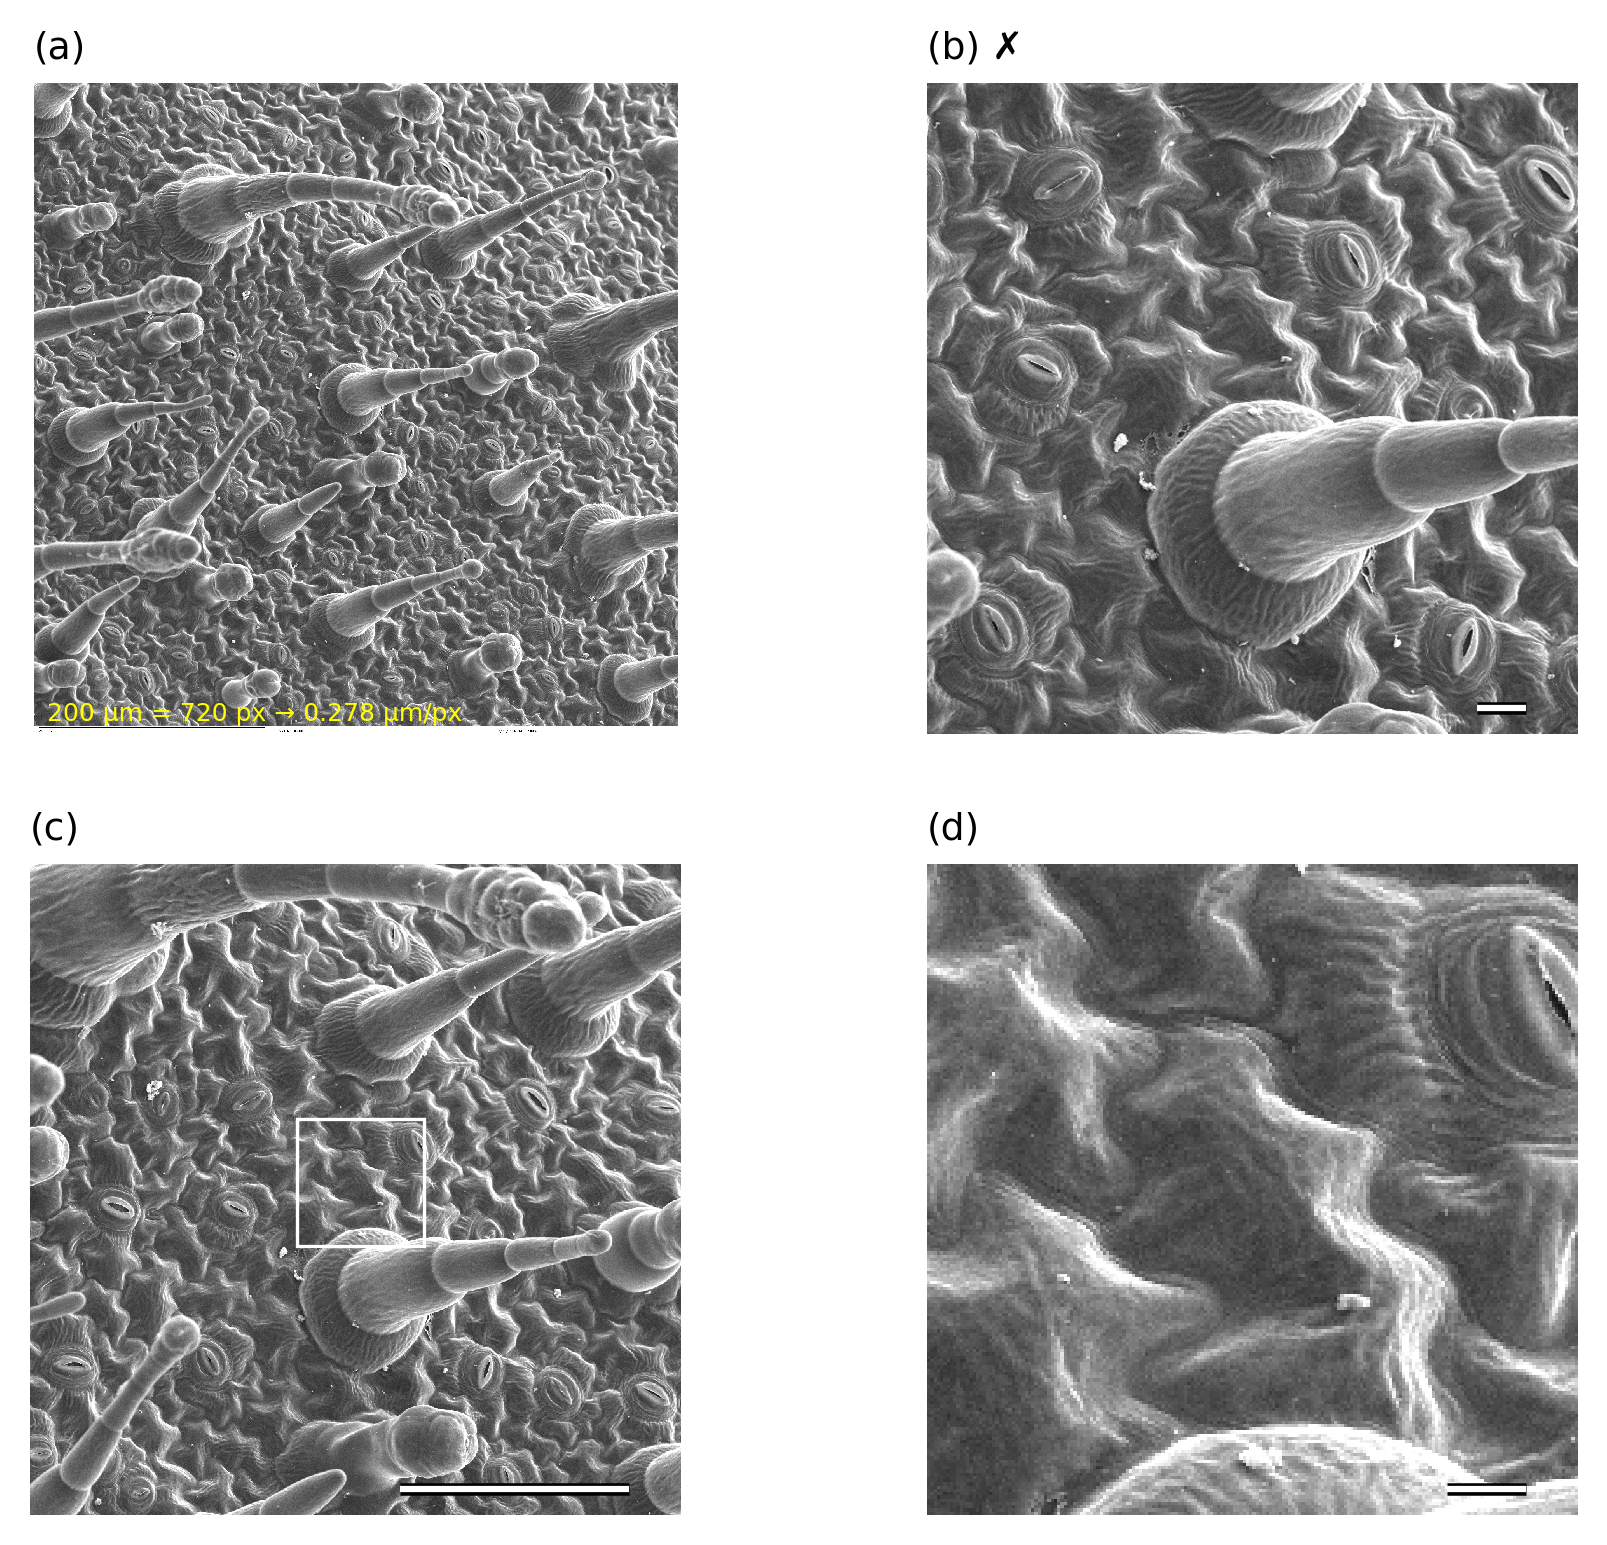
\includegraphics[width=0.88\linewidth]{figures/ch08/ch08-05-crop-inset-scalebar-en.png}
\caption{Cropping, insets and scale bars. (a) Original SEM image (\emph{Nicotiana alata} upper leaf epidermis; Zeiss~962, $200\times$) with the instrument data bar; its $200\ \mu\text{m}$ line spans $720$ pixels, giving $0.278\ \mu\text{m}$ per pixel. (b) Counter-example: data bar removed, a single structure kept, enlarged with bicubic interpolation, and a scale bar drawn without any basis. (c) Recommended: the crop box is recorded and a $100\ \mu\text{m}$ scale bar is drawn from the pixel size; the boxed region is enlarged $3\times$ by nearest-neighbour sampling in (d), scale bar $20\ \mu\text{m}$. Image: Louisa Howard, Dartmouth Electron Microscope Facility, public domain.}\label{fig:ch08-05}
\end{figure}

Comparing the four panels of Figure~\ref{fig:ch08-05} shows how each step is verified:
\begin{itemize}
\item \textbf{Panel (a) (measuring pixel calibration from the instrument data bar):} The bottom $25$ pixel rows (rows $2048\text{--}2072$) form the white data bar generated by the Zeiss DSM~962 SEM, containing a black scale line and the text ``\texttt{200 um},'' ``\texttt{200X},'' ``\texttt{7/31/3 REMF},'' and ``\texttt{Nict.\ leaf \#2.001}.'' Scanning the data bar programmatically for the longest horizontal run of dark pixels (grey value $< 80$) locates the black scale line at rows $2052\text{--}2053$, $x = 15\text{--}734$, spanning exactly \textbf{$720$ pixels}. This gives $s_{\text{px}} = 200\ \mu\text{m} / 720\ \text{px} \approx 0.2778\ \mu\text{m/px}$ (reliant on the microscope's magnification calibration, so the legend states that the scale bar is derived from the instrument data bar). Wikimedia Commons also hosts a third-party derivative (\path{Leaf_epidermis_w_scale.jpg}, $2048 \times 2052$ pixels) with the data bar cropped off and a white ``$200\ \mu\text{m}$'' bar added. Third-party scale bars must always be checked against the primary file: measuring that derivative's white line ($x = 240\text{--}959$) confirms it is $720$ pixels long, matching the original data bar.
\item \textbf{Panel (b) (counter-example):} The data bar is discarded, a single trichome ($600 \times 600$ pixels) is upscaled $4\times$ with bicubic interpolation, and an unverified ``$50\ \mu\text{m}$'' bar is drawn at twice the true calibrated length.
\item \textbf{Panels (c) and (d) (recommended practice):} Panel~(c) logs a $1024 \times 1024$-pixel crop at $(480, 320)\text{--}(1504, 1344)$, draws a calibrated $100\ \mu\text{m} = 360\ \text{px}$ scale bar, and marks a $200 \times 200$-pixel stomatal region at $(900, 720)\text{--}(1100, 920)$ in white; panel~(d) enlarges that box $3\times$ with nearest-neighbour sampling and recalculates the scale bar as $20\ \mu\text{m} = 72 \times 3 = 216\ \text{px}$.
\end{itemize}

\subsection{No Calibration, No Scale Bar}

When an image lacks both calibration metadata and an instrument data bar, the only compliant choice is to \textbf{omit the scale bar and state in the legend that the pixel size is unknown}---never guessing from ``how big a cell usually looks.''

Figure~\ref{fig:ch08-06} shows a three-channel fluorescence micrograph from the NIH ImageJ sample set (\path{FluorescentCells.jpg}, bovine pulmonary artery endothelial cells stained with blue DAPI, green microtubules, and red F-actin; public domain, $512 \times 512$ pixels; also an example of the red/green merge issue from Section~3). Published as an 8-bit lossy JPEG composite with a unitless $1:1$ JFIF density and no objective or pixel size recorded on Commons or the ImageJ source page (panel~a), adding an eyeballed scale bar (panel~b) fabricates scale. Omitting the bar and stating ``pixel size unknown'' in the legend (panel~c) is the honest course. Enlarging the patch $(200, 200)\text{--}(280, 280)$ by $4\times$ with nearest-neighbour sampling (panel~d) exposes $8 \times 8$ JPEG compression blocks and cross-channel bleeding, confirming that the file is a display derivative rather than raw measurement data.

\begin{figure}[htbp]\centering
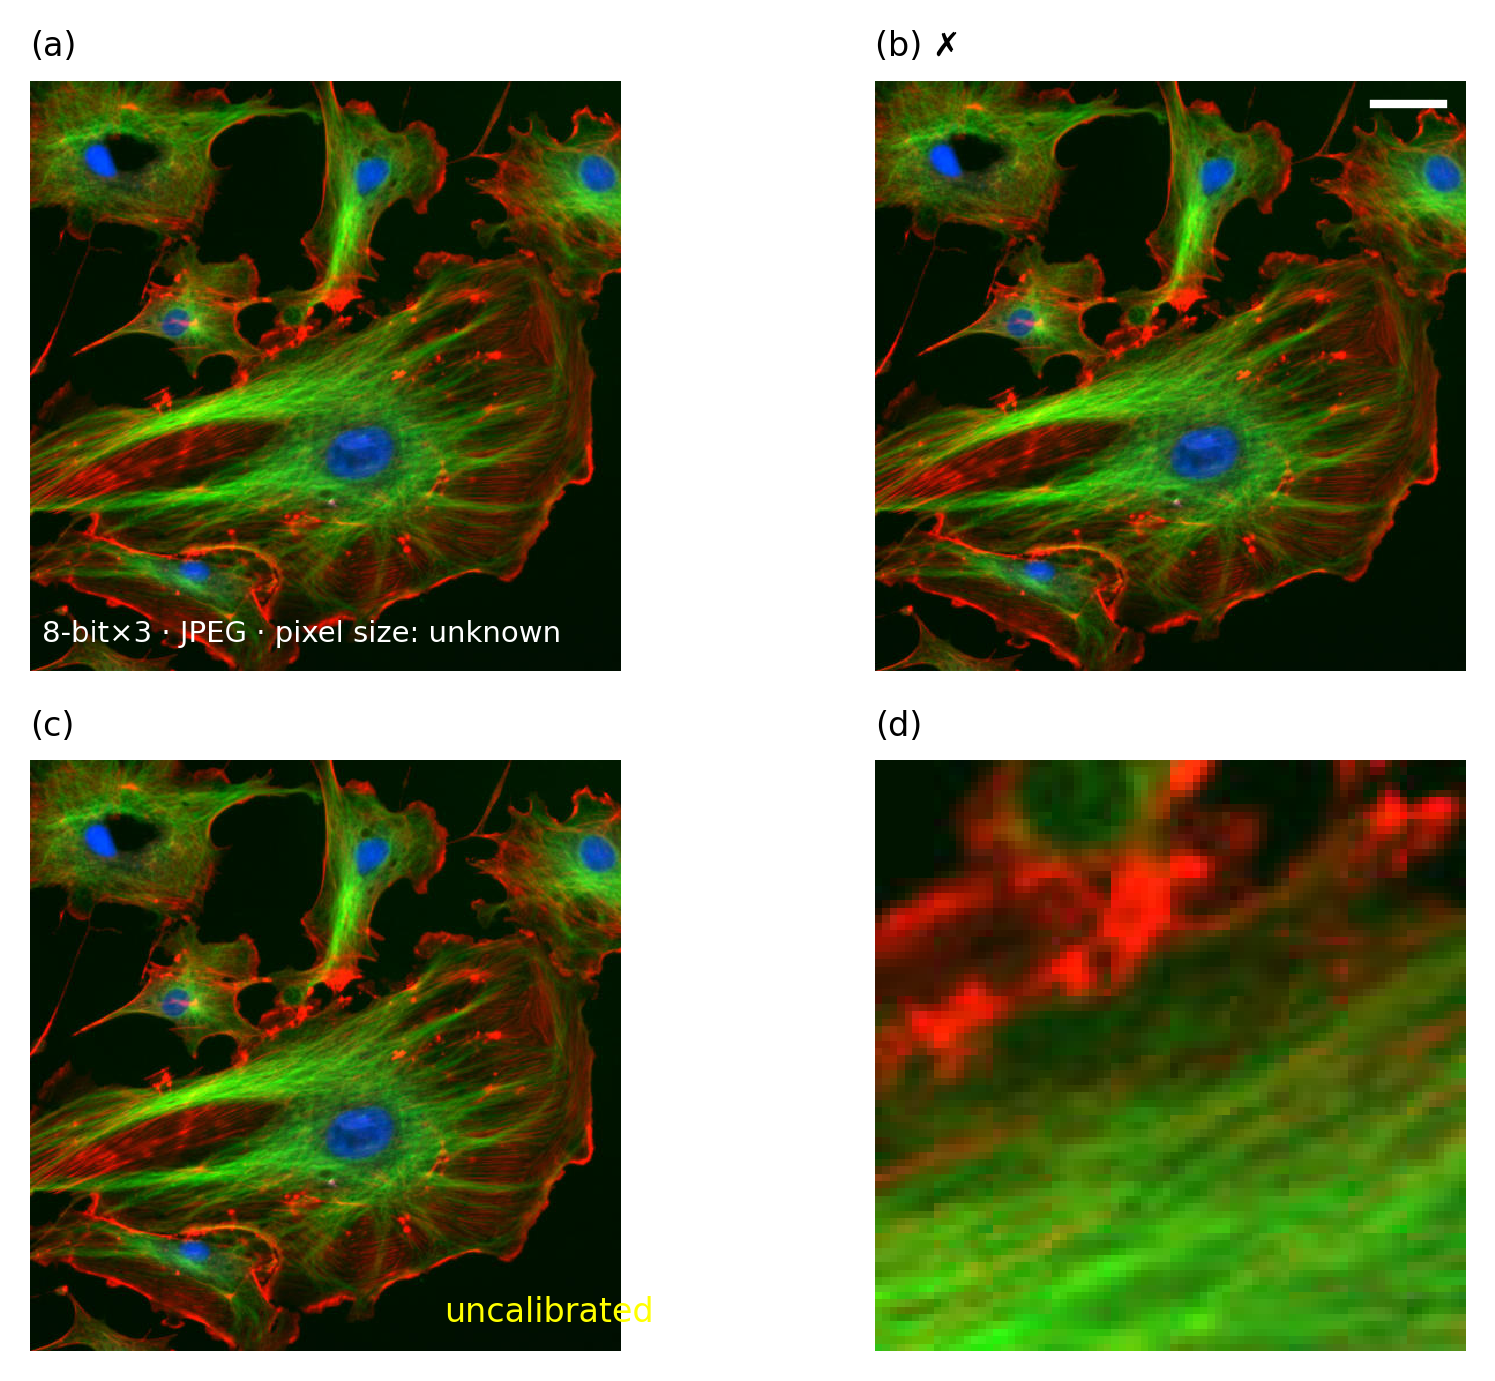
\includegraphics[width=0.88\linewidth]{figures/ch08/ch08-06-no-calibration-en.png}
\caption{No calibration, no scale bar. (a) A three-channel fluorescence image from the ImageJ sample set (bovine pulmonary artery endothelial cells; blue DAPI, green microtubules, red F-actin), published as an 8-bit JPEG composite with no recorded pixel size. (b) Counter-example: a scale bar added by guesswork. (c) Recommended: no scale bar, and the legend states that the pixel size is unknown. (d) Enlargement reveals JPEG compression blocks: the file is a display image, not raw measurement data. Image: public domain (Wikimedia Commons, FluorescentCells.jpg).}\label{fig:ch08-06}
\end{figure}

\section{Journal Rules and the Boundaries of AI}

The \emph{Journal of Cell Biology} guidelines (Rossner and Yamada, 2004) and Cromey's (2010) ethical rules established the baseline for scientific digital images: whole-image adjustments to brightness, contrast, or colour balance are acceptable (with non-linear adjustments disclosed in the caption), but \textbf{no specific feature within an image may be enhanced, obscured, moved, removed, or introduced}. Bik et al.\ (2016) screened $20,621$ biomedical papers and found inappropriate image duplication or manipulation in $3.8\%$, prompting publishers to adopt automated pre-publication image forensics.

In the generative AI era, the Nature Portfolio \emph{Image Integrity and Standards} policy and the Springer Nature \emph{Artificial Intelligence (AI)} policy (both accessed 2026-10-29; because publisher policies evolve rapidly, authors must verify current wording before submission) reinforce these rules: adjustments must be applied across the whole image and equally to controls, must not eliminate data, must disclose pseudo-colouring, non-linear ($\gamma$) mappings, and per-channel adjustments in merges, prohibit clone and healing tools, and classify \textbf{``fabrication of data, citations, or results'' and ``generation of photorealistic images (deepfakes)'' as impermissible}.

Why does passing a blurry micrograph to a generative model to ``denoise and sharpen'' count as fabricating data? We tested this with a ground-truth experiment on the \emph{Nicotiana alata} SEM micrograph from Figure~\ref{fig:ch08-05} (Figure~\ref{fig:ch08-07}):
\begin{enumerate}
\item Crop a $512 \times 512$-pixel patch $(640, 680)\text{--}(1152, 1192)$ from the original SEM image as \textbf{ground truth (GT, panel~a)}, containing three stomata, epidermal cell ridges, the base of a large right trichome, and a small lower-left trichome.
\item Downsample $4\times$ by $4 \times 4$ area averaging to produce a $128 \times 128$-pixel low-resolution input \textbf{LR (panel~b, nearest-neighbour display)}.
\item \textbf{Control~1 (panel~c):} Upscale LR back to $512 \times 512$ pixels with deterministic bicubic interpolation (blurry, but adds no new structures).
\item \textbf{Control~2 (panel~d):} Pass the same $128 \times 128$ LR image to an image-generation model in image-editing mode three independent times with a typical naive user prompt (to avoid cherry-picking the worst run, panel~d shows Run~1 and Runs~2 and~3 are archived):
\end{enumerate}

\begin{Prompt}
Upscale this grayscale scanning electron microscope image to 512 x 512 pixels.
Make it sharper and more detailed, remove blur and noise, and enhance the fine
surface structures so it looks like a high-resolution micrograph.
Keep it grayscale. Do not add any text, letters, numbers, labels, or scale bars.
Square 1:1 aspect ratio.
\end{Prompt}

\begin{figure}[htbp]\centering
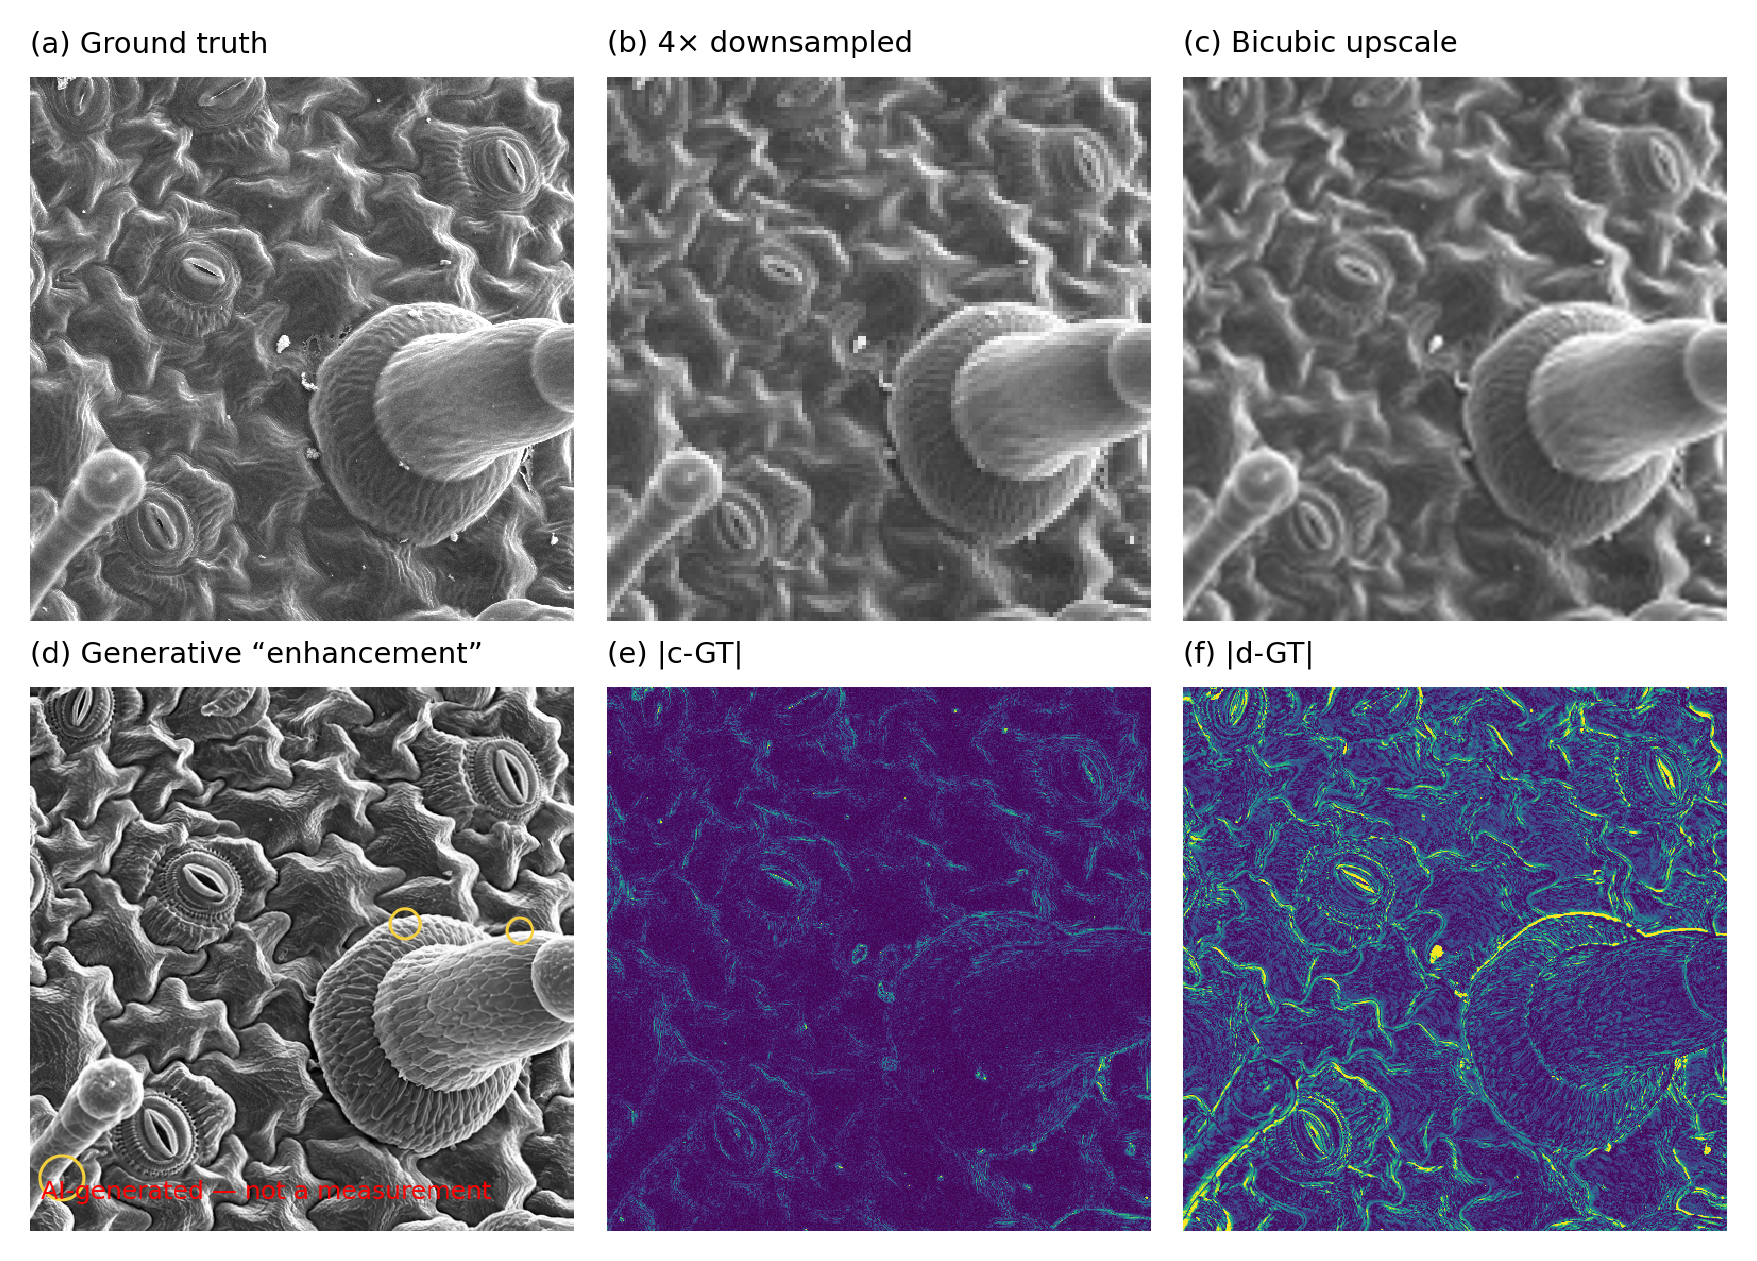
\includegraphics[width=0.88\linewidth]{figures/ch08/ch08-07-generative-risk-en.png}
\caption{Generative ``enhancement'' invents structure. (a) Crop of the original SEM image (ground truth). (b) The same crop downsampled $4\times$. (c) Bicubic upscaling: blurry, but nothing new is added. (d) Upscaling by an image-generation model asked to ``make it sharper and more detailed'': it looks crisper yet contains edges and textures absent from the original (circles). (e, f) Absolute differences of (c) and (d) from the original. The generated image illustrates the risk only and must never be used as experimental data. Original: Louisa Howard, Dartmouth Electron Microscope Facility, public domain; panel (d) was generated by an image model (prompt and generation log in the book repository).}\label{fig:ch08-07}
\end{figure}

Comparing the six panels of Figure~\ref{fig:ch08-07} and the three runs reveals four distortions common to any generative upscaler:
\begin{itemize}
\item \textbf{Loss of control over dimensions and channel mode:} Although the prompt requested a $512 \times 512$ single-channel greyscale image, all three runs returned $1254 \times 1254$-pixel ($9.8\times$) three-channel 8-bit RGB files with inter-channel spreads up to $10\text{--}12$ grey levels.
\item \textbf{Fabricated anatomical boundaries and textures:} Panel~(d) looks sharper than bicubic upscaling (c), but comparison against ground truth (a) reveals invented multi-ringed collars and serrated teeth around the upper-left stomatal pore, plus dense scale-like striations across the right trichome and cuticle. At the three yellow circles on panel~(d)---two crease ridges on the upper basal collar of the large trichome (near $(353, 222)$ and $(460, 229)$) and the tip of the lower-left trichome (near $(30, 461)$)---the model hallucinated bright rims and boundaries absent from the specimen.
\item \textbf{Contradictory details across repeated runs:} From the exact same $128 \times 128$ input, Run~1 synthesized tight scale-like strips, Run~2 produced rounded pebble-like granules and split the lower-left trichome tip into polygonal blocks, and Run~3 drew radiating pleats around the large trichome base---proving these high-frequency details are stochastic texture synthesis rather than specimen measurements.
\item \textbf{Pixel-wise error nearly triple that of bicubic interpolation:} Converting Run~1 to greyscale, resizing to $512 \times 512$ with Lanczos solely for comparison, and applying rigid registration ($-0.5^\circ$ rotation, $dx = -1, dy = +1$ pixel) yields the difference maps in panels~(e) and~(f) (shared $0\text{--}128$ \texttt{viridis} scale). Bicubic interpolation $|c - \text{GT}|$ (panel~e) has a mean absolute error (MAE) of $10.32$ grey levels, whereas generative upscaling $|d - \text{GT}|$ (panel~f) reaches an MAE of $28.91$ after registration ($29.06$ before registration).
\end{itemize}

The conclusion is absolute: \textbf{AI can help you write processing scripts, draft methods, and check colour vision, but it must never generate a single pixel that will be treated as a measurement.}

\section{Complete Case Study: Presenting Control-Field Images of U2OS Cells}

We now walk through Su's supplementary methods figure from raw TIFFs to verified delivery. Supplementary Figure~S1 shows the nuclear and mitochondrial staining patterns of U2OS cells under DMSO control (\texttt{mock}) conditions so peers can judge raw image quality for downstream profiling. It \textbf{reports no treatment effect}, and because it uses the benchmark dataset BBBC022v1 (Gustafsdottir et al., 2013), acquisition parameters cite the dataset documentation ($20\times$ objective, $0.656\ \mu\text{m/pixel}$) and primary paper without inventing unrecorded settings.

\textbf{Step~1: Build the raw-image catalogue (Deliverable~1).} Lock the four 16-bit TIFFs for well A13 sites \texttt{s1} and \texttt{s2} as read-only, verify SHA-256 hashes by script, and generate the raw-image catalogue (Table~\ref{tab:ch08-catalog} and companion CSV).

\begin{table}[htbp]\centering\footnotesize
\setlength{\tabcolsep}{3pt}
\renewcommand{\arraystretch}{1.15}
\caption{Raw-image catalogue for the case study (site~1 channels shown; site~2 \texttt{w1} spans $122\text{--}1450$, mean $227.1$, $p_{0.1}/p_{99.9}=129/1150$, and \texttt{w5} spans $176\text{--}1655$, mean $366.3$, $p_{0.1}/p_{99.9}=196/1078$, logged in the companion CSV).}\label{tab:ch08-catalog}
\begin{tabularx}{\linewidth}{@{}>{\raggedright\arraybackslash}p{25mm}YY@{}}
\toprule
\textbf{Field} & \textbf{Example: s1 Hoechst (w1)} & \textbf{Example: s1 MitoTracker (w5)} \\
\midrule
Filename & \path{IXMtest_A13_s1_w1B35C6D5D-DBF9-4779-990D-5E7AFB14D600.tif} & \path{IXMtest_A13_s1_w5B257EE32-37B0-4698-891B-11B1B3D3D0C1.tif} \\
Source & BBBC022v1, plate 20585, well A13 (\texttt{mock}), site~1 & BBBC022v1, plate 20585, well A13 (\texttt{mock}), site~1 \\
Channel / dye & w1 / Hoechst 33342 (DNA) & w5 / MitoTracker Deep Red (mitochondria) \\
Dimensions / depth & $696 \times 520\ \text{px}$, 16-bit container, 12-bit effective & $696 \times 520\ \text{px}$, 16-bit container, 12-bit effective \\
Pixel size & $0.656\ \mu\text{m}$ (dataset docs, $20\times$) & $0.656\ \mu\text{m}$ (dataset docs, $20\times$) \\
SHA-256 (first 16) & \texttt{4be40f814481002a} (full 64-hex in CSV) & \texttt{c1c441e44e91481c} (full 64-hex in CSV) \\
Raw value range & $121\text{--}1655$; $p_{0.1}/p_{99.9}=132/1236$; saturated: $0$ & $185\text{--}4095$; $p_{0.1}/p_{99.9}=218/1140$; saturated: $12$ \\
License \& status & CC0 1.0; read-only master, processed on copies & CC0 1.0; read-only master, processed on copies \\
\bottomrule
\end{tabularx}
\end{table}

\textbf{Step~2: Write the figure brief (Deliverable~2).} Write the brief below in your own document and save it; you will refer to it after choosing ``Multi-panel figure'' in the \scidraw{} Scientific Figure Workflow wizard (\sdtool{figure-workflow}) and following the route into the Multi-Panel Figure Maker (\sdtool{multi-panel-figure-maker}):

\begin{Prompt}
[Purpose & Audience] Supplementary methods figure (Supplementary Fig. S1), double-column
width 174 mm; for cell-imaging peers evaluating raw image and staining quality.
[Goal] Show nuclear (Hoechst 33342) and mitochondrial (MitoTracker Deep Red) staining
patterns of U2OS cells under DMSO control conditions; no treatment effect is reported.
[Source Material] BBBC022v1 (CC0), plate 20585, well A13 (mock), site s1; channels w1, w5;
16-bit TIFF, 696 x 520 px, 0.656 um/pixel (dataset docs). Originals read-only; SHA-256 logged.
[Panels] a, Nuclei (greyscale); b, Mitochondria (greyscale); c, Merge (nuclei magenta,
mitochondria green); d, Enlarged inset of a subregion in c (marked by a white box on c).
[Allowed Processing] Whole-image linear display mapping (black/white points), pseudo-colour
LUT, cropping, integer-multiple nearest-neighbour enlargement. One display range per channel
shared across all panels and written to the processing log.
[Prohibited] Gamma or curves, denoising, sharpening, deconvolution, background subtraction,
local adjustments, or any generative "enhancement".
[Scale Bars & Selection] From 0.656 um/pixel: 50 um on a-c, recalculated 10 um on d; white
solid bars at bottom right, length stated in legend. Select a typical cell near field median
intensities for d; report the 12 saturated pixels (4095) in w5 without retouching.
[Export & Verification] Lossless 8-bit PNG panels assembled in SciDraw AI Multi-Panel Figure
Maker (TIFF/PDF + log); trace SHA-256, verify scale bars and deuteranopia separability.
\end{Prompt}

\textbf{Step~3: Use a general-purpose AI assistant to organize the presentation plan and draft the processing script.} Submit the following prompt to a general-purpose AI chat assistant to generate the plan and deterministic Python script:

\begin{Prompt}
I have two raw 16-bit fluorescence micrographs and need a supplementary methods figure.
Before writing code, outline a presentation plan: what each panel shows, whether each step
is a linear operation, and what must be disclosed in the processing log and figure legend.
Images: two 16-bit greyscale TIFFs, 696 x 520 px; w1 = Hoechst 33342 (nuclei),
w5 = MitoTracker Deep Red (mitochondria); pixel size 0.656 um (dataset documentation);
effective 12-bit camera data, with 12 saturated pixels (4095) in w5.
Requirements:
1. Use whole-image linear display mapping only; set black/white points by raw percentiles.
2. Merge with magenta (nuclei) and green (mitochondria), explaining why red/green is avoided.
3. Compute scale-bar lengths in pixels from 0.656 um/px, recalculating for the zoomed inset.
4. List prohibited operations (denoising, sharpening, gamma, local edits, generative upscale).
5. List every item I must verify manually.
Once the plan is confirmed, write a Python script that reads the originals read-only and saves
display ranges, crop coordinates, zoom factor, scale-bar pixels, and SHA-256 to processing-log.json.
\end{Prompt}

Never copy percentile thresholds or pixel lengths estimated in chat prose; let the script compute them directly on the real 16-bit TIFF arrays and write them to \path{processing-log.json}. Run the script on a copy first and inspect the code to confirm no denoising, sharpening, or gamma functions are called.

\textbf{Step~4: Audit the five flaws in the first draft (\texttt{v1}) and issue a revision order.} Figure~\ref{fig:ch08-08} shows an ad hoc first draft counter-example with five numbered flaws:
\begin{enumerate}
\item \textbf{Issue~1 (auto-contrast per panel):} Panels~\textbf{a} and~\textbf{b} are stretched separately to their own \texttt{min--max}, and the merge in~\textbf{c} uses another mapping, leaving no unified parameters to report.
\item \textbf{Issue~2 (red--green merge):} Panel~\textbf{c} merges red and green, which become hard to distinguish under simulated red--green colour-vision deficiency.
\item \textbf{Issue~3 (unfounded scale bar):} The ``$20\ \mu\text{m}$'' bar at the bottom right of~\textbf{c} is $50\ \text{px}$ long, whereas at $0.656\ \mu\text{m/px}$ a true $20\ \mu\text{m}$ bar is $30.5\ \text{px}$---$64\%$ too long.
\item \textbf{Issue~4 (brightest cell + bicubic interpolation):} Inset~\textbf{d} cherry-picks the brightest, most atypical condensed nucleus in the field (coordinates $x = 488\text{--}552$, $y = 184\text{--}248$), upscales it $4\times$ with bicubic interpolation, and omits a locator box on~\textbf{c}.
\item \textbf{Issue~5 (undisclosed $\gamma = 0.6$ and lossy export):} The mitochondrial channel applies an undisclosed $\gamma = 0.6$ boost and exports as a quality-70 JPEG.
\end{enumerate}

\begin{figure}[htbp]\centering
\resizebox{0.88\linewidth}{!}{% FIG ch08-08 v1 issue overlay (English).
% Numbered marks sit on the panel each problem belongs to.
% The phrases are listed under the micrograph so they do not cover it.
\tikzset{%
  chviiiissue/.style={%
    circle, draw=BookInk, line width=0.4pt, fill=white, inner sep=0.2pt,%
    minimum size=9pt, font=\sffamily\fontsize{7}{8}\selectfont, text=BookInk%
  },%
  chviiicap/.style={%
    anchor=west, inner xsep=0.4pt, inner ysep=0.5pt,%
    font=\sffamily\fontsize{7}{9}\selectfont, text=BookInk%
  }%
}
\providecommand{\chviiimark}[1]{%
  \tikz[baseline=(n.base)]{\node[chviiiissue] (n) {#1};}%
}
\begin{tikzpicture}
  \node[anchor=south west, inner sep=0pt] (img) at (0,0)
    {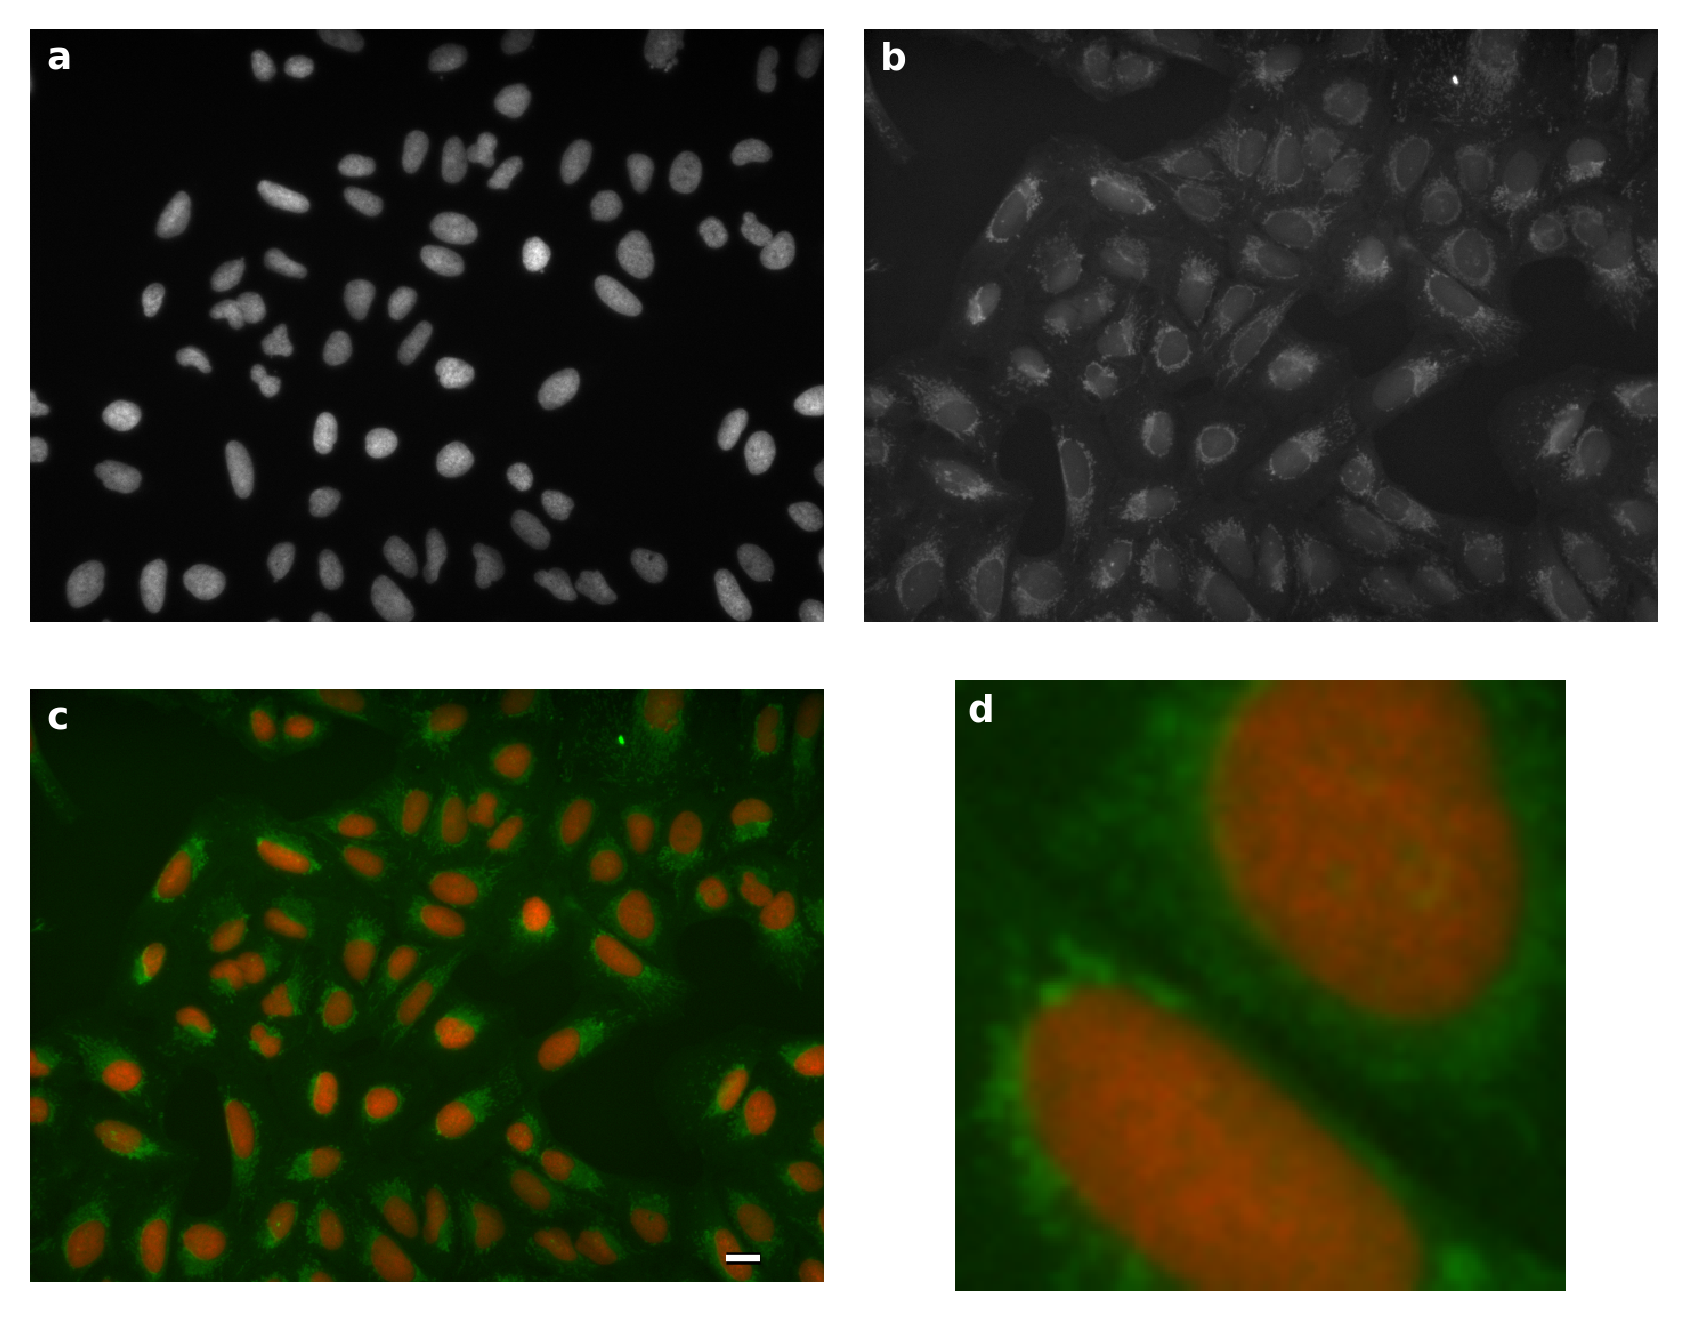
\includegraphics[width=\linewidth]{figures/ch08/ch08-08-case-v1-en.png}};
  \begin{scope}[x={(img.south east)}, y={(img.north west)}]
    \node[chviiiissue] (m1) at (0.40, 0.92) {1};
    \node[chviiiissue] (m2) at (0.40, 0.45) {2};
    \node[chviiiissue] (m3) at (0.36, 0.09) {3};
    \draw[BookInk, line width=0.35pt] (0.372, 0.078) -- (0.424, 0.056);
    \node[chviiiissue] (m4) at (0.88, 0.12) {4};
    \node[chviiiissue] (m5) at (0.90, 0.92) {5};
  \end{scope}
  \node[chviiicap] (c1) at ([yshift=-1.8mm]img.south west)
    {\chviiimark{1}\enspace auto-contrast per panel};
  \node[chviiicap] (c2) at ([yshift=-0.8mm]c1.south west)
    {\chviiimark{2}\enspace red--green};
  \node[chviiicap] (c3) at ([yshift=-0.8mm]c2.south west)
    {\chviiimark{3}\enspace unfounded scale bar};
  \node[chviiicap] (c4) at ([yshift=-0.8mm]c3.south west)
    {\chviiimark{4}\enspace brightest cell + bicubic};
  \node[chviiicap] (c5) at ([yshift=-0.8mm]c4.south west)
    {\chviiimark{5}\enspace undisclosed $\gamma=0.6$};
\end{tikzpicture}
}
\caption{Five common problems in a first draft (numbered 1--5; see text). This version was produced deliberately with wrong settings as a teaching counter-example. The legend for the final version is given in the case section.}\label{fig:ch08-08}\label{fig:ch08-08-v1}
\end{figure}

Against these five flaws, we issue an itemized revision order:

\begin{Prompt}
Revision Order (v1 -> final)
1. Fix one linear display range per channel across all panels:
   Hoechst black point 132, white point 1236 (raw p0.1 / p99.9);
   MitoTracker black point 218, white point 1140 (raw p0.1 / p99.9). Share in the merge.
2. Remove gamma; use strictly linear mapping and log "linear_no_gamma: true".
3. Change merge LUT to magenta nuclei (R+B) and green mitochondria (G); verify under
   deuteranopia and protanopia simulation.
4. Recalculate scale bars from 0.656 um/pixel: 50 um = 76.2 px (panels a-c);
   for panel d (3x nearest-neighbour enlargement), 10 um = 15.24 px x 3 = 45.7 px.
5. Move the inset crop in d to a representative cell near median nuclear and mitochondrial
   intensities at pixel coordinates (280, 328)-(344, 392); draw a white locator box on c.
6. Enlarge d by 3x using nearest-neighbour sampling only (no bicubic or "detail enhancement").
7. Export lossless 8-bit PNG panels; archive raw 16-bit TIFFs, script, and processing-log.json.
8. Disclose in both processing log and legend that 12 pixels in w5 saturated at acquisition (4095).
\end{Prompt}

\textbf{Step~5: Assemble in the \scidraw{} Multi-Panel Figure Maker, merge the two-tier processing logs, and complete verification.} Once the script generates four lossless 8-bit PNG panels and \path{processing-log.json}, open the \scidraw{} Multi-Panel Figure Maker (\sdtool{multi-panel-figure-maker}): import the four panels, choose a double-column preset ($174\ \text{mm}$ width, such as Cell or Springer), set a $2 \times 2$ grid with automatic labels \textbf{a}--\textbf{d} (any in-tool cropping or rotation is also logged), and export the ZIP package (TIFF, PNG, PDF, PPTX, and assembly log) to produce the final figure (Figure~\ref{fig:ch08-09}).

\begin{figure}[htbp]\centering
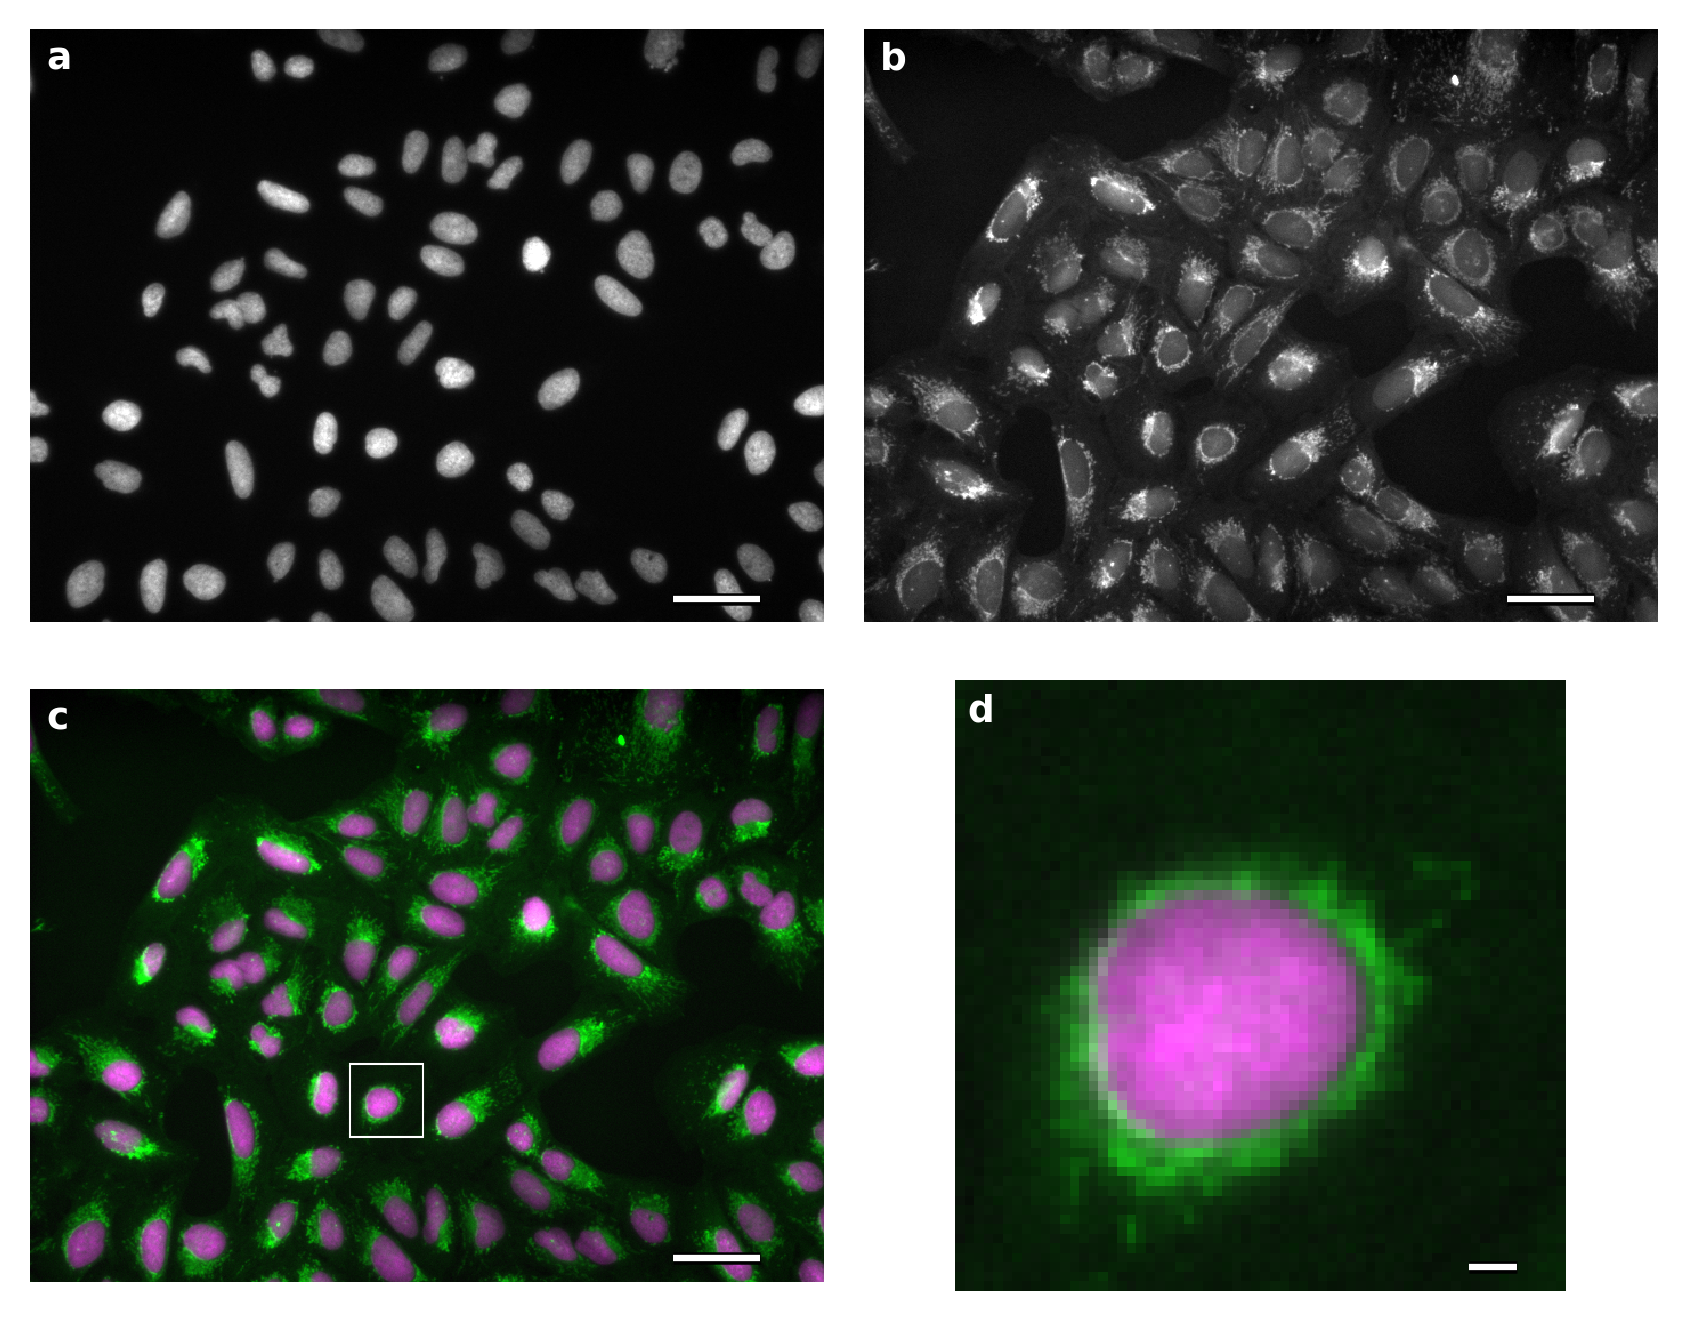
\includegraphics[width=0.88\linewidth]{figures/ch08/ch08-08-case-final-en.png}
\caption{Supplementary Fig.\ S1 | Nuclear and mitochondrial staining of U2OS cells under DMSO control conditions. \textbf{a}, Hoechst~33342 (nuclei). \textbf{b}, MitoTracker Deep Red (mitochondria). \textbf{c}, Merge (nuclei magenta, mitochondria green); the white box marks the region shown in~\textbf{d}. \textbf{d}, The boxed region in~\textbf{c} enlarged $3\times$ with nearest-neighbour sampling. Images are from BBBC022v1 (plate 20585, well A13, site~1; CC0; Gustafsdottir et al., 2013), acquired with a $20\times$ objective at $0.656\ \mu\text{m}$ per pixel. All panels use whole-image linear display mapping with no gamma or other non-linear adjustment; display ranges were $132\text{--}1236$ (Hoechst) and $218\text{--}1140$ (MitoTracker) in raw 12-bit values and are identical for each channel across panels. Twelve pixels in the mitochondrial channel were saturated at acquisition ($4095$) and were not altered. Scale bars, $50\ \mu\text{m}$ (\textbf{a}--\textbf{c}) and $10\ \mu\text{m}$ (\textbf{d}). Raw 16-bit images, the processing script and the processing log are provided as Supplementary Data.}\label{fig:ch08-09}\label{fig:ch08-08-final}
\end{figure}

At this step, the author must verify two critical platform boundaries:
\begin{enumerate}
\item \textbf{Merge the upstream processing log with the multi-panel assembly log:} The assembly log exported by \sdtool{multi-panel-figure-maker} records each panel's filename, SHA-256 hash, original dimensions and bit depth, crop box, rotation or flip, physical millimetre width, effective resolution, and resampling mode, and states: ``Apart from the cropping, rotation, and scaling recorded above, no brightness, contrast, colour, or content modifications were applied to any panel.'' Crucially, \textbf{this statement covers only operations inside the multi-panel tool.} Because the imported PNG panels already underwent upstream intensity mapping and pseudo-colour merging in the script---and because the multi-panel tool currently does not generate calibrated scale bars, channel labels, or linked inset boxes, nor does its ZIP bundle the raw 16-bit TIFFs---the author must \textbf{merge} the script's \path{processing-log.json} with the assembly log into one complete processing record so readers are not misled into thinking no display adjustment occurred.
\item \textbf{Check effective resolution honestly and complete the figure legend:} A $696\ \text{px}$-wide raw image spans about $59\ \text{mm}$ at $300\ \text{dpi}$; in a $174\ \text{mm}$-wide $2 \times 2$ grid where each panel is roughly $85\ \text{mm}$ wide, the effective resolution is about $208\ \text{dpi}$. Authors must either accept this lower effective resolution and state the native pixel dimensions transparently, or reduce the panel width to reach $300\ \text{dpi}$---\textbf{never upscaling by interpolation to fake higher resolution}. Next, run the Figure Checker (\sdtool{figure-checker}) to check file format, resolution, greyscale contrast, and colour-vision risks (noting that it performs technical checks rather than scientific review), and use the Figure Legend assistant (\sdtool{figure-legend}) to draft a description of visible features before manually adding fluorophores, pixel size, display windows, saturation counts, and scale-bar lengths (by design, the tool never invents magnification, scale bars, or methods).
\end{enumerate}

\begin{Prompt}
Supplementary Fig. S1 | Nuclear and mitochondrial staining of U2OS cells under DMSO control
conditions. a, Hoechst 33342 (nuclei). b, MitoTracker Deep Red (mitochondria). c, Merge
(nuclei magenta, mitochondria green); the white box marks the region shown in d. d, The
boxed region in c enlarged 3x with nearest-neighbour sampling. Images are from BBBC022v1
(plate 20585, well A13, site 1; CC0; Gustafsdottir et al., 2013), acquired with a 20x
objective at 0.656 um per pixel. All panels use whole-image linear display mapping with no
gamma or other non-linear adjustment; display ranges were 132-1236 (Hoechst) and 218-1140
(MitoTracker) in raw 12-bit values and are identical for each channel across panels. Twelve
pixels in the mitochondrial channel were saturated at acquisition (4095) and were not
altered. Scale bars, 50 um (a-c) and 10 um (d). Raw 16-bit images, the processing script
and the processing log are provided as Supplementary Data.
\end{Prompt}

\begin{table}[htbp]\centering\footnotesize
\setlength{\tabcolsep}{3pt}
\renewcommand{\arraystretch}{1.15}
\caption{Verification audit for the final case-study figure (Supplementary Fig.\ S1).}\label{tab:ch08-verify}
\begin{tabularx}{\linewidth}{@{}>{\raggedright\arraybackslash}p{25mm}YY@{}}
\toprule
\textbf{Verification item} & \textbf{Audit method} & \textbf{Measured result} \\
\midrule
Input file hashes & Script asserts SHA-256 of four panels against catalogue & Matches Table~\ref{tab:ch08-catalog} and catalogue CSV; originals unmodified \\
Display range \& linearity & Cross-check \path{processing-log.json} against figure legend & Hoechst $132\text{--}1236$, MitoTracker $218\text{--}1140$, linear with no $\gamma$, 12 saturated pixels reported \\
Scale-bar pixel lengths & Recompute from $0.656\ \mu\text{m/px}$ and measure on exported figure & Panels \textbf{a}--\textbf{c}: $50\ \mu\text{m} = 76.2\ \text{px}$; panel \textbf{d} ($3\times$): $10\ \mu\text{m} = 45.7\ \text{px}$; exact match \\
Inset \& crop coordinates & Compare white box on \textbf{c} with crop coordinates of \textbf{d} & Shared median-cell coordinates $(280, 328)\text{--}(344, 392)$, $3\times$ nearest-neighbour sampling \\
Colour vision \& log merge & Machado (2009) simulation, \sdtool{figure-checker}, and dual-log check & Magenta/green separable under red--green deficiency; upstream and assembly logs merged \\
\bottomrule
\end{tabularx}
\end{table}

\section{What AI Can and Cannot Do in Presenting Experimental Images}

Table~\ref{tab:ch08-01} summarizes the boundaries between AI tools and author verification across each step of experimental image presentation.

\begin{table}[htbp]\centering\scriptsize
\setlength{\tabcolsep}{3pt}
\renewcommand{\arraystretch}{1.08}
\caption{What AI can do, what AI cannot do, and what the author must verify when presenting experimental images.}\label{tab:ch08-01}
\begin{tabularx}{\linewidth}{@{}>{\raggedright\arraybackslash}p{20mm}YYY@{}}
\toprule
\textbf{Stage} & \textbf{What AI can do} & \textbf{What AI cannot do} & \textbf{What the author must verify} \\
\midrule
Raw-image cataloguing & Draft catalogue templates; write scripts to read metadata and compute SHA-256 hashes & Judge which file on disk is truly raw; fill in missing acquisition settings & Originals read-only; hashes match catalogue; acquisition parameters have documented sources \\
Presentation planning & List panel processing steps and required disclosures; separate linear from non-linear steps & Decide which field of view is representative; interpret biological meaning & Selection rationale, complete controls, and compliance with journal rules \\
Display mapping & Write scripts to set percentile black/white points uniformly across panels and output parameters & Automatically ``tune until it looks good''; adjust local regions separately & Identical settings across compared panels; no data-destroying clipping; non-linear steps disclosed \\
Pseudo-colour & Recommend colourblind-safe combinations; write simulation scripts; \sdtool{figure-checker} checks colour risk & Guarantee all readers can distinguish channels; replace split-channel greyscale & Magenta/green or split greyscale; simulation check results; colour mapping stated in legend \\
Cropping \& insets & Write scripts logging crop boxes and zoom factors; multi-panel tool logs crop, rotation, scale, and effective dpi & Invent details absent from the original; ``super-resolve'' evidentiary images & Unbiased selection; nearest-neighbour sampling or declared interpolation; adequate effective dpi \\
Scale bars & Compute scale-bar pixel lengths from calibrated pixel size & Estimate pixel size without calibration; infer physical scale from image content & Pixel-size provenance (metadata, data bar, or micrometer); recalculated after magnification \\
Enhancement \& restoration & None---generative models are never used on the pixel path of evidentiary images & Denoise, sharpen, inpaint, remove artefacts, or ``make blurry images crisp'' & Zero generative operations; deterministic processing (e.g., deconvolution) fully specified \\
Legends \& methods & \sdtool{figure-legend} drafts visible descriptions; assistant drafts methods text from processing logs & Invent fluorophores, objectives, pixel sizes, or sample sizes & Source, license, display settings, saturation note, and scale-bar lengths complete \\
\bottomrule
\end{tabularx}
\end{table}

\section{Chapter Checklist}

\begin{itemize}
\item Store original raw files as read-only and record filename, source, bit depth, dimensions, physical pixel size, SHA-256 hash, and license in the raw-image catalogue.
\item Apply all display adjustments across the whole image; use identical display settings across all panels in a comparison and log the numerical parameters.
\item Confirm that no valid data are obliterated by clipping and report any pixels saturated at acquisition.
\item Disclose any non-linear adjustments ($\gamma$, curves, or logarithmic transforms) explicitly in the figure legend.
\item Use colourblind-friendly pseudo-colour combinations (such as magenta/green) or split-channel greyscale panels for multichannel images, and verify with colour-vision simulations.
\item Document a written selection basis for cropped regions, mark inset boxes on the parent image, and state the magnification factor and interpolation method.
\item Ensure scale-bar lengths can be recomputed from the physical pixel size; when calibration information is unavailable, omit the scale bar and state that pixel size is unknown in the legend.
\item Never splice images from different fields, time points, or samples into a single continuous field; separate juxtaposed panels with clear dividing lines and explain them in the legend.
\item Confirm that not a single pixel of any evidentiary image has been processed by generative AI.
\item Merge the multi-panel tool's assembly log with the upstream processing log, and archive the raw 16-bit files and scripts for Supplementary Data.
\end{itemize}

\section{Exercises}

\begin{enumerate}
\item \textbf{Evaluating processing steps (pen and paper).} For each of the following six descriptions---(1) ``brightening the treated panel separately so faint structures are visible''; (2) ``applying $\gamma = 0.8$ uniformly across an entire merged image and stating it in the legend''; (3) ``removing a dust speck with the clone-stamp tool''; (4) ``placing cells from two fields into the same panel without a dividing line''; (5) ``setting a linear display range at the $0.1\text{th}/99.9\text{th}$ percentiles and applying it uniformly across all panels''; (6) ``upscaling a JPEG screenshot to $4\text{K}$ with a generative AI tool''---classify the step as \emph{Acceptable}, \emph{Acceptable with disclosure}, or \emph{Unacceptable}, and cite the rules in Section~5 to justify your choice (reference answers in the Appendix).
\item \textbf{Scale-bar calculation (scripting).} Download \path{Leaf_epidermis.jpg} (Wikimedia Commons), write a script to measure the pixel length of the scale line in the bottom instrument data bar, and calculate the physical pixel size; draw a $100\ \mu\text{m}$ scale bar on a $600 \times 600\ \text{px}$ crop; then enlarge that crop $2\times$ using nearest-neighbour interpolation and recalculate the scale bar. Compare your results with the values in this chapter ($720\ \text{px}$, $0.278\ \mu\text{m/px}$) and state what assumption this pixel size relies on.
\item \textbf{Hands-on with \scidraw{}.} Using the four final panels generated by this chapter's script, choose ``Multi-panel figure'' in the Scientific Figure Workflow wizard (\sdtool{figure-workflow}) and follow step 1, ``Lay out panels'', into the Multi-Panel Figure Maker (\sdtool{multi-panel-figure-maker}): choose a $174\ \text{mm}$ double-column preset, a $2 \times 2$ grid, and automatic panel numbering; export the ZIP package; open the processing record, find the statement that ``no brightness, contrast, colour, or content modifications were applied,'' write a short paragraph explaining why that sentence alone is incomplete for this figure, and merge the script's \path{processing-log.json} into a unified processing note. Finally, inspect the exported figure with \sdtool{figure-checker} and record what it reports and what it does not check.
\end{enumerate}

\section*{References}

\begin{itemize}\sloppy
\item Bik EM, Casadevall A, Fang FC. The prevalence of inappropriate image duplication in biomedical research publications. \emph{mBio}. 2016;7(3):e00809-16. doi:10.1128/mBio.00809-16
\item Crameri F, Shephard GE, Heron PJ. The misuse of colour in science communication. \emph{Nature Communications}. 2020;11:5444. doi:10.1038/s41467-020-19160-7
\item Cromey DW. Avoiding twisted pixels: ethical guidelines for the appropriate use and manipulation of scientific digital images. \emph{Science and Engineering Ethics}. 2010;16(4):639--667. doi:10.1007/s11948-010-9201-y
\item Gustafsdottir SM, Ljosa V, Sokolnicki KL, et al. Multiplex cytological profiling assay to measure diverse cellular states. \emph{PLoS ONE}. 2013;8(12):e80999. doi:10.1371/journal.pone.0080999
\item Jambor H, Antonietti A, Alicea B, et al. Creating clear and informative image-based figures for scientific publications. \emph{PLOS Biology}. 2021;19(3):e3001161. doi:10.1371/journal.pbio.3001161
\item Ljosa V, Sokolnicki KL, Carpenter AE. Annotated high-throughput microscopy image sets for validation. \emph{Nature Methods}. 2012;9(7):637. doi:10.1038/nmeth.2083
\item Machado GM, Oliveira MM, Fernandes LAF. A physiologically-based model for simulation of color vision deficiency. \emph{IEEE Transactions on Visualization and Computer Graphics}. 2009;15(6):1291--1298. doi:10.1109/TVCG.2009.113
\item Rossner M, Yamada KM. What's in a picture? The temptation of image manipulation. \emph{Journal of Cell Biology}. 2004;166(1):11--15. doi:10.1083/jcb.200406019
\item Schmied C, Jambor HK. Effective image visualization for publications -- a workflow using open access tools and concepts. \emph{F1000Research}. 2020;9:1373. doi:10.12688/f1000research.27140.1
\item Wong B. Points of view: Color blindness. \emph{Nature Methods}. 2011;8(6):441. doi:10.1038/nmeth.1618
\item Broad Bioimage Benchmark Collection. BBBC022v1 image set (U2OS Cell Painting). \url{https://bbbc.broadinstitute.org/BBBC022} (accessed 2026-10-29).
\item Nature Portfolio. Editorial policies: Image integrity and standards. \url{https://www.nature.com/nature-portfolio/editorial-policies/image-integrity} (accessed 2026-10-29).
\item Nature Portfolio / Springer Nature. Editorial policies: Artificial Intelligence (AI). \url{https://www.nature.com/nature-portfolio/editorial-policies/ai} (accessed 2026-10-29).
\item Okabe M, Ito K. Color Universal Design (CUD): How to make figures and presentations that are friendly to colorblind people. \url{https://jfly.uni-koeln.de/color/} (accessed 2026-10-29).
\end{itemize}
